\documentclass[twocolumn,a4paper,10pt]{article}

\usepackage[utf8]{inputenc}
\usepackage[english]{babel}
\usepackage[T1]{fontenc}
%%%%%% MISE EN PAGES %%%%%%
\usepackage[width=175mm, top=3cm]{geometry}

\setcounter{tocdepth}{3}     % Dans la table des matieres
\setcounter{secnumdepth}{4}  % Avec un numero.

% \renewcommand{\chaptermark}[1]{\markboth{\thechapter.\space#1}{}} 
\usepackage{layout}

%%%%%% SYMBOLES %%%%%
\usepackage{tipa}	% pour avoir l'accent concave
\usepackage{lmodern}	% pour les guillemets
\usepackage{nth}

%%%%%% EQUATION %%%%%%
\usepackage{amssymb}
\usepackage{amsmath}
\usepackage{fancybox}
\usepackage{xfrac}	% fraction de type "1/4"
\usepackage{cases}	% système équation
\usepackage[overload]{empheq}
\usepackage{bm}		% pour mettre en gras .
\usepackage{units} 	% x/y barre latérale pour les fractions

%%%%%% FIGURE %%%%%%
\usepackage{graphicx}	% insérer des graphiques
\usepackage{subfigure}	% utiliser subfigure
\usepackage{float}	% utiliser H dans les figures

%%%%%% TABLEAUX %%%%%%
\usepackage{array,multirow,makecell}
%\addto\captionsfrench{\def\tablename{\textsc{Tableau}}}% pour avoir TABLEAU et pas TABLE dans les légendes des tableaux
\usepackage[table,xcdraw]{xcolor} % pour avoir des lignes colorées dans les tableau
\usepackage{slashbox} % pour les \backslashbox
%\usepackage{subcaption}
\usepackage{hhline}	% pour les lignes horizontales 
\usepackage{tabularx} % permet itemize dans les cellules


\newcolumntype{L}[1]{>{\raggedright\let\newline\\\arraybackslash\hspace{0pt}}m{#1}}
\newcolumntype{C}[1]{>{\centering\let\newline\\\arraybackslash\hspace{0pt}}m{#1}}
\newcolumntype{R}[1]{>{\raggedleft\let\newline\\\arraybackslash\hspace{0pt}}m{#1}}

%%%%%%%%%%%%%%%%%%%%%
\usepackage{url}	% gérer les adresses www.
\linespread{1}	% interligne

\cleardoublepage

\newcommand{\ml}[1]{\textcolor{blue}{ Mathieu: #1}}

\title{Estimation of the road traffic sound levels based on Non-Negative Matrix Factorization}

\author{
    Jean-Rémy GLOAGUEN\\
    Arnaud Can\\
    LAE\\
    Ifsttar\\
    jean-remy.gloaguen@ifsttar.fr
  \and
    Mathieu Lagrange\\
	Jean-François Petiot \\
    LS2N, CNRS\\
    \'Ecole Centrale de  Nantes\\
}
\date{}
\begin{document}

\maketitle

\section*{Abstract}

\section{Introduction}
\subsection{Related work}
With the introduction of the European Directive 2002/EC/49, cities over 100 000 inhabitants have to produce road traffic noise maps. These maps depict an estimation of the number of city dwellers exposed to high noise levels and to draw up action plans to reduce it as too long exposures to these noises can generate health problems \cite{who_burden_2017}. These maps are the result of a simulation process based on the estimation of the traffic density on the main roads and the use of sound propagation techniques. They express $L_ {DEN}$ and $L_N$, which are \textit{Day-Evening-Night} and \textit{Night} equivalent A-weighted sound levels respectively. However, these maps introduce lot of uncertainty generated by the numerical tools \cite{van_leeuwen_noise_2015}, by the different calculation methodologies used \cite{leroy_uncertainty_2010}\cite{garg_critical_2014} or even by the calculation procedure of the number of inhabitants exposed to noise \cite{king_implementation_2011}. In addition, the usual road traffic noise maps are static, aggregating the exposure on the two indicators $L_{DEN}$ and $L_N$, thus ignoring the sound levels evolution throughout the day. Since the creation of road traffic noise maps entails long data collection and calculation times, the use of acoustic measurements could facilitate their updating or even the generation of dynamic maps \cite{wei_dynamic_2016}. These measurements can be performed at fixed stations spread all over the cities \cite{Mioduszewski} \cite{mietlicki2012innovative}, which would lead to the availability of the long-term evolution of the traffic noise levels. It can also be performed with  mobile stations \cite{can_exploring_2012} \cite{manvell2004sadmam} covering a larger area with fewer sensors but also sparse time periods. 

Currently, sensor networks in cities are spread for multiple applications (air quality assessment, measurement of meteorological parameters, ...), including the assessment of urban noise levels. DYNAMAP project \cite{dynamap_2016} studied the deployment and feasibility of such installations. It focuses on sensor installations on specific roads at the city scale in Milan and Rome \cite{bellucci_life_2017}. In a similar way, but reduced to few neighborhoods, the CENSE project\footnote{\url{http://cense.ifsttar.fr/}} \cite{picaut2017characterization} aims to combine \textit{in situ} observations, from a sensor network, and numerical data, from noise modeling, through data assimilation techniques.

If sensors networks could improve road traffic noise estimation compared with simulated maps, the issue of the correct estimation from  measurements of the traffic sound level is still unsolved \cite{Mioduszewski}. Indeed, the urban sound environment is a complex environment gathering lots of different sounds (car passages, voices, bird's whistles, car horn \dots) that can overlap. Consequently, the traffic sound level estimation based on measurements is also not a trivial task.
Many recent works have focused on the detection or recognition tasks of environmental sounds without distinction between them\cite{heittola_sound_2011}, \cite{defreville_automatic_2006}, \cite{dufaux_automatic_2000}, \cite{chu_environmental_2009}. A two step process is generally followed : describe the audio files with a set of features (Spectrum Gravity Spectrum, harmonicity, Mel-Frequency Cepstral Coefficient \dots) and classify them with the help of classifiers (Support Vector Machines, Gaussian Mixture Models, Hidden Markov Model, Artifical Neural Networks). A description of there features and classifiers can be found in \cite{cowling_comparison_2003} and their application can be found in \cite{shen_environmental_2012}, \cite{beritelli_pattern_2008}, \cite{couvreur_automatic_2004}.

Recently, an Anomalous Noise Events Detector has been generated in \cite{socoro_anomalous_2017} to detect the sound sources from labeled recordings that are not related to the traffic component in order not to take them into account on the estimation of the traffic sound level. If the detection of the road traffic noise is good, the detection of these anomalous noise events stay weak and no information on the improvement on the estimation of the traffic  level are presented. Furthermore, this work and as well as the other works in the detection or recognition tasks, do not address the overlap of environmental sounds in an urban context. Although near major roads or ring roads traffic is predominant on all other sound sources, there are many places where road traffic overlaps with other sound sources that contribute significantly to the overall sound levels. In such case, the only detection of the traffic component does not make it possible to determine precisely its noise level.

In consequence, to be effective on a wide range of sound environments, we propose in this paper to follow the blind source separation paradigm. That is, separating the contribution of the traffic from the other sources within a polyphonic scene.

\ml{tu passe beaucoup de temps a taper sur socoro et peu a parler de ton approche. Ce n'est pas une bonne pratique. Je dirais ils font ca, nous aussi on fait ca c'est super, et nous on le fais comme ca, regardez tout ce que ca permet (et implicitement eux ils peuvent pas).}

\ml{tu plonges tres vite dans la technique}

One of the first and the most widely \ml{faux} used techniques to do so is the Independent Component Analysis \cite{comon_independent_1994}. The principle is to decompose $N$ recorded signals to a sum of $P$ independent sound sources weighted by linear relations. This method is most of all suited for the 'cocktail party' issue where one tries to capture a signal among noise.  However, ICA is limited to only over determined cases ($N > P$). Furthermore, if it is suited for indoor environments where the number of sound sources is constant, it can not be fitted for an outdoor environment where the number of sources is unknown and variable and, moreover, it would be necessary to mount multiples sensors on one point to perform the source separation \ml{je ne vois pas ou est le probleme, il y a des gens qui le font}. A more convenient method is Non-negative Matrix Factorization (NMF) \cite{lee_learning_1999} which consists in approximating the magnitude spectrogram of an audio file from the product of two matrices. It has been widely used in the audio domain, \cite{smaragdis_non-negative_2003} \cite{wilson_speech_2008} \cite{mesaros_sound_2015}, and has already been employed for the source separation task of monaural signals of speech and music \cite{wang_musical_2005} \cite{wilson_speech_2008}. By design, this method deals reasonably well with the overlaping sound sources as soon as the overlap can be resolved on the time/frequency plane. For the environmental sounds, the method has been used for the geo-localisation and classification of the sound environment, like in \cite{kumar_audio_2016} where NMF is used to classify the audio files according to the 10 cities where they have been recorded. It has also been used by Innami and Kasai in the unsupervised case \cite{satoshi_innami_nmf-based_2012} for source separation. They proposed a source separation in two steps by separating the sound background from the events first and by separating the events between them. The audio files tested results of a simulation process where a sound background (river or wind) are added to two sound events (school chime, announcement, frog croaking, dog barging and bell ringing).

 If the method proposed is interesting, the main issue here is the small size of the database (only 9 sounds) on which the algorithms are tested while some sounds (frog and river) are not representative of sounds that can be found in cities.
 \ml{encore une fois, utilise la critique implicite. On peut tout critiquer, surtout un papier qui n'est pas encore publié, fais attention. faire une liste des contributions avec 1) 2) 3) et finir par un paragraphe de structure}

\subsection{Proposed approach}

\ml{tu melange contribution technique et protocole experimental, ca va pas. pas de soussection a l'intro}

We propose in this paper a method based on the Non-Negative Matrix Factorization (NMF) technique to estimate the global, $\tilde{L}_{p,traffic}$, and the 1-s equivalent, $\tilde{p}_{1s,traffic}$ sound level of the traffic through the supervised and the semi-supervised approaches as well as a method using thresholding. To validate these approaches, we consider a corpus of simulated scenes artificially created with the simulator software \textit{simScene}. The use of simulated sound scenes is necessary as it offers a full control on the design of the scenes and the knowledge of the exact contribution of the traffic component which would hardly be extracted from a recording of an urban scene ($L_{p,traffic}$ and $p_{1s,traffic}$). Both the sound scene simulation and NMF require the creation of two sound databases; see Figure \ref{fig:blocDiagramNMF}. In parallel, a baseline method built from a frequency low-pass filter is computed. This method considers that road traffic is mainly composed of low frequencies and therefore can be filtered by a low-pass filter at the cut-off frequency $f_c$; see Figure \ref{fig:blocDiagramFilter}. The performance of the frequency low-pass filter and NMF are then compared with the calculation of two metrics (Mean Absolute Error, normalized Root Mean Square Error).

\begin{figure*}[t]
\centering
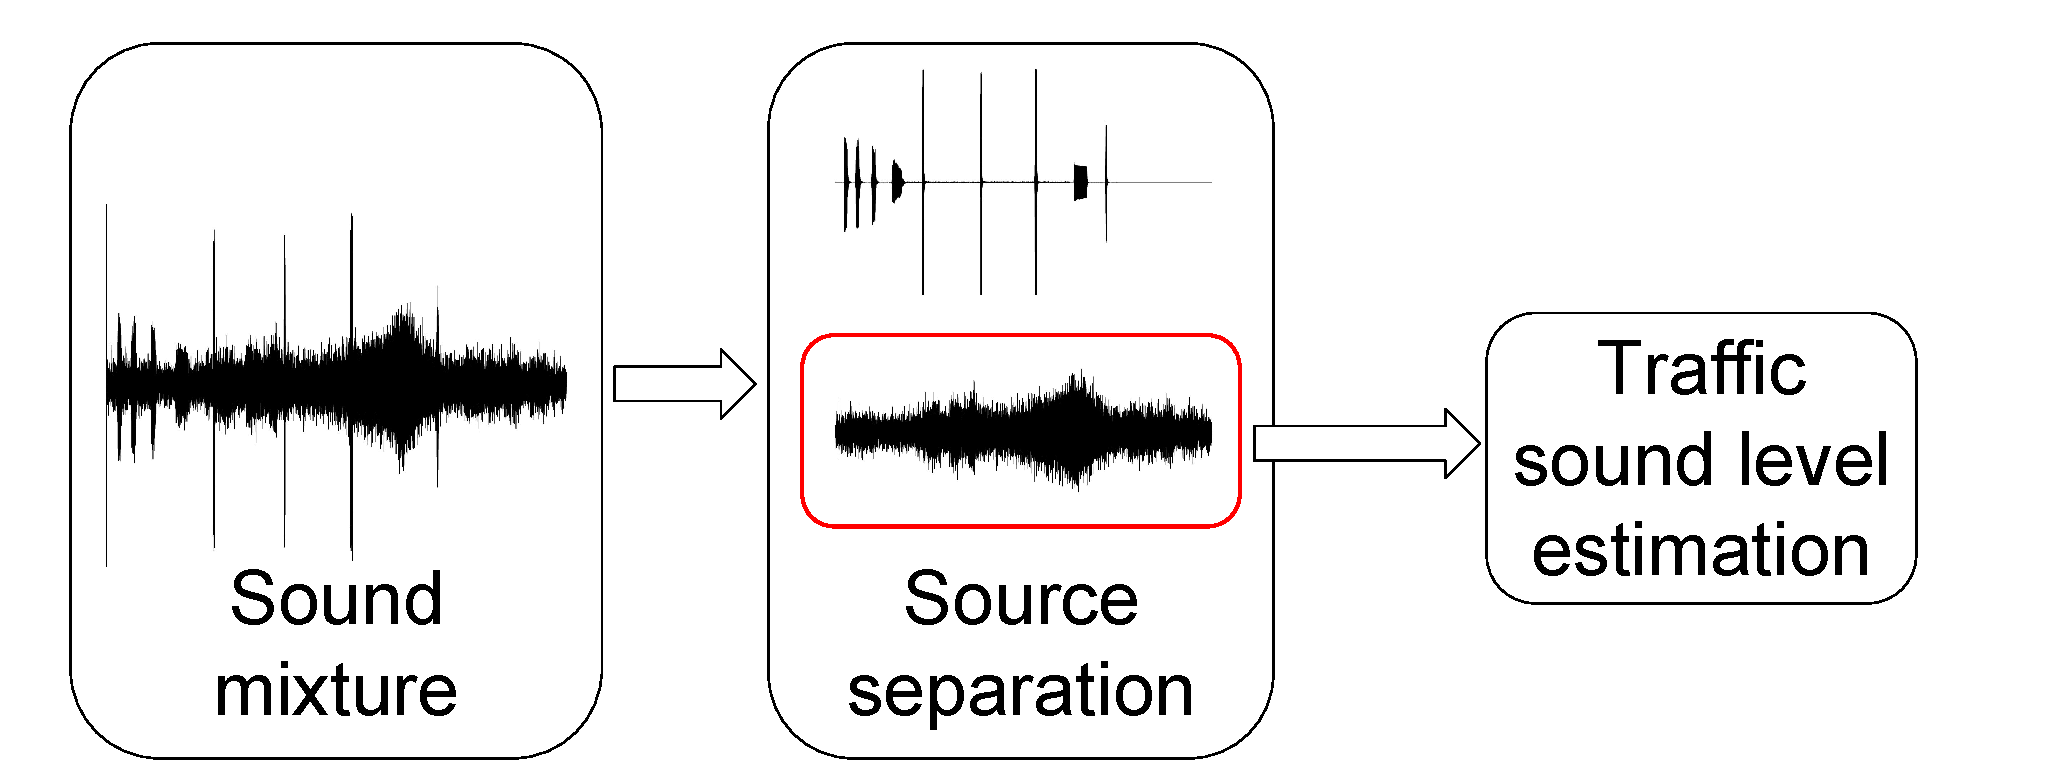
\includegraphics[width=0.7\textwidth]{figures/bloc_diagram_source_separation.pdf}
\caption{Bloc diagram of the source separation method}
\end{figure*}

The remaining of the paper is organized as follows. Section \ref{part:nmf} details the technical aspect of NMF. Section \ref{part:protocol} described on the design of the environmental sound scene corpus and the experimental protocol setup. Then Section \ref{part:results} shows and discusses the results obtained during the parametric study.

The experience is lead with the Matlab software. In order to be a reproductive experience, all the programs\footnote{\url{https://github.com/jean-remyGloaguen/article2017EstimationAmbiance}} and the sound database\footnote{\url{https://sandbox.zenodo.org/record/176695#.Wk4ow3kiGos}} (TEMPORAIRE) used are available online.

\section{Non-negative Matrix Factorization}\label{part:nmf}
\subsection{Description of NMF}
Non-negative Matrix Factorization is a matrix approximation method introduced by Lee and Seung, \cite{lee_learning_1999}, which can be used to approximate the spectrogram (obtained using a Short-Term Fourier Transform) of an audio file, $\mathbf{V}$, $\in \mathbb{R}^+_{F \times N}$ as :

\begin{equation}\label{eq:nmf}
\mathbf{V} \approx \mathbf{\tilde{V}} = \mathbf{WH}
\end{equation}

where $\mathbf{W} \in \mathbb{R}^+_{F \times K}$ is the \textit{dictionary} (or basis) matrix composed of audio spectrum and $\mathbf{H} \in \mathbb{R}^+_{K \times N}$ is the \textit{activation} matrix which summarizes the temporal evolution of each element of $\mathbf{W}$. An illustrative example can be found in Figure  \ref{fig:example_NMF}.

\begin{figure}[t]
\centering
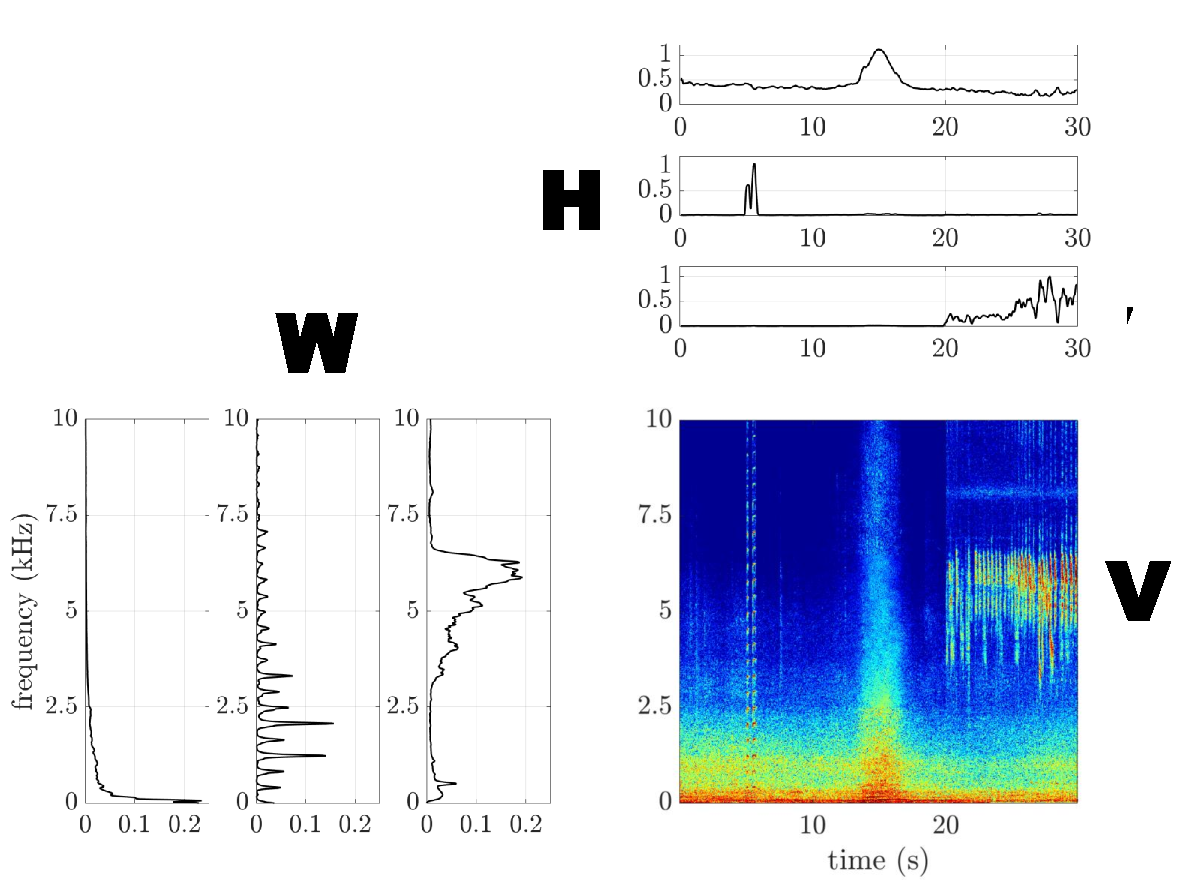
\includegraphics[width=0.9\linewidth]{figures/schema_introduction_nmf.pdf}
\caption{Example of a simple NMF  for urban sound mixture, $\mathbf{W}$ and $\mathbf{V}$ are composed of 3 elements (car passages, car horn and bird's whitles)}
\label{fig:example_NMF}
\end{figure}

The choice of the dimensions is often made as that $F\times K + K \times N < F \times N$. NMF is then considered as a low rank approximation method. However, this constraint is not essential. To estimate the quality of the approximation, an objective function is used

\begin{equation}\label{eq:min-D-WH}
\underset{\mathbf{H} \geq 0, \mathbf{W} \geq 0}{\min} D\left(\mathbf{V} \vert \vert \mathbf{\tilde{V}}\right).
\end{equation}

The operator $D(x\vert y)$ is a divergence calculation such as:
\begin{equation}
D\left(\textbf{V} \vert\vert \mathbf{\tilde{V}} \right) = \sum_{f = 1}^{F} \sum_{n = 1}^{N} d_{\beta}
\left(\textbf{V}_{fn} \vert \left[ \textbf{WH} \right]_{fn} \right)
\end{equation}

and usually belongs to the $\beta-$divergence class \cite{fevotte_nonnegative_2009} in which the well known Euclidean distance (eq. \ref{eq:def_distEUC}) and the Kullback-Leibler divergence (eq. \ref{eq:def_divKL}) belong

\begin{subequations}\label{eq:divBetaGenerale}
\begin{numcases}{d_{\beta}(x\vert y) =}
    \frac{1}{2}(x-y)^2, & $\beta = 2$, \label{eq:def_distEUC}\\
    x\log \dfrac{x}{y} - x + y, & $\beta = 1$.\label{eq:def_divKL}
\end{numcases}
\end{subequations}

Prior knowledge on the content can be adjusted with the addition of constraints (like the smoothness or the sparsness criteria \cite{virtanen_monaural_2007}) in the objective function , see equation (\ref{eq:min-D-WH}), to better take account prior knowledge of the sources.

Algorithms have been proposed to solve the minimization problem (\ref{eq:min-D-WH}) iteratively such as the multiplicative update \cite{lee_algorithms_2000}, the alternating least square method \cite{cichocki_regularized_2007}, the projected gradient \cite{lin_projected_2007} \dots Here, the multiplicative update is chosen as it ensure non-negative results of which convergence has been proved \cite{fevotte_algorithms_2011}.

\subsection{Supervised NMF}
First, supervised NMF is used: the \textit{dictionary} includes audio spectrum of urban sound sources as, in the urban environments, a lot of different sound sources present are known and their spectrum can be obtained. The \textit{basis} are then the unknown to estimate. In the first iteration, $\mathbf{H}$ is initialized randomly, then it is updated by the generic algorithm

\begin{equation}\label{eq:updateH_Sup}
\textbf{H}^{(i+1)} \leftarrow \textbf{H}^{(i)}.\left(\frac{\textbf{W}^T \left[\left(\textbf{WH}^{(i)} \right)^{(\beta-2)}.\textbf{V} \right]}{\textbf{W}^T \left[\textbf{WH}^{(i)} \right]^{(\beta-1)}}\right)^{\gamma(\beta)}
\end{equation}

with $\gamma(\beta) = \frac{1}{2-\beta},$ for $\beta < 1$, $ \gamma(\beta) = 1$, for $\beta \in \left[1,2\right]$ and $\gamma(\beta) = \frac{1}{\beta-1}$ for $\beta > 2$. The product $A.B$ and $A/B$ symbolized the Hadamard product and ratio. As in the supervised approach, the position in $\mathbf{W}$ of traffic component is known, the source separation of this sound source is made by extracting the dictionary and basis elements related,

\begin{equation}\label{eq:separationExtraction}
\mathbf{\tilde{V}}_{traffic} = \left[ \mathbf{WH} \right]_{traffic}.
\end{equation}

\subsection{Semi-supervised NMF}

One of the main issue with the supervised approach is the generalization issue: how to be adapted to different sound mixtures with a fixed dictionary ? To better take into account the diverse nature of urban scenes, semi-supervised NMF can be useful as it has been proposed \cite{lee_semi-supervised_2010} to offer more flexibility. This method consists in composing the \textit{dictionary} with a fixed part $\mathbf{W_s} \in \mathbb{R}^+_{F\times K}$, composed in our case of spectrum representative of road traffic and with a mobile part, $\mathbf{W_r} \in \mathbb{R}^+_{F\times J}$ with $J <<K$, that is updated. Here, $J = 2$. The aim is to include in $\mathbf{W_r}$ the element that are not related with the traffic. The problem (\ref{eq:nmf}) become

\begin{equation}
\mathbf{V} \approx \mathbf{W_s H_s}+ \mathbf{W_r H_r}.
\end{equation}

In a similar way as to solve the equation \ref{eq:min-D-WH}, $\mathbf{W_r}$, $\mathbf{H_r}$ and $\mathbf{H_s}$ are successively updated with the relations (\ref{eq:WH-SSupdate}):

{\scriptsize
\begin{subequations}\label{eq:WH-SSupdate}
\begin{align}
\mathbf{W_r}^{(i+1)} &\leftarrow \mathbf{W_r}^{(i)}.\left(\frac{\left[\left(\mathbf{W_r H_r}^{(i)} \right)^{(\beta-2)}.\mathbf{V} \right]\mathbf{H_r}^T}{\left(\mathbf{W_r H_r}^{(i)} \right)^{(\beta-1)}\mathbf{H_r}^T}\right)^{\gamma(\beta)}, \label{eq:W_r_SS}\\
\mathbf{H_r}^{(i+1)} &\leftarrow \mathbf{H_r}^{(i)}.\left(\frac{\mathbf{W_r}^T \left[\left(\mathbf{W_r H_r}^{(i)} \right)^{(\beta-2)}.\mathbf{V} \right]}{\mathbf{W_r}^T \left(\mathbf{W_r H_r}^{(i)} \right)^{(\beta-1)}}\right)^{\gamma(\beta)}, \label{eq:H_r_SS}\\
\mathbf{H_s}^{(i+1)} &\leftarrow \mathbf{H_s}^{(i)}.\left(\frac{\mathbf{W_s}^T \left[\left(\mathbf{W_s H_s}^{(i)} \right)^{(\beta-2)}.\mathbf{V} \right]}{\mathbf{W_s}^T \left(\mathbf{W_s H_s}^{(i)} \right)^{(\beta-1)}}\right)^{\gamma(\beta)}.\label{eq:H_s_SS}
\end{align}
\end{subequations}}

\subsection{Thresholded initialized NMF}

A last approach is tested based on unsupervised NMF. Usually, $\mathbf{W}$ is learnt with the help of a learning corpus by initiated it randomly. Here, as the concerned sound source is known and audio samples of car passages are available, a initial dictionary, $\mathbf{W_0}$, is learnt by converting the audio files in the spectra domain; see part \ref{part:dictionary_learning}). Then NMF is performed where $\mathbf{W}$ (eq. \ref{eq:updateW_unsup}) and $\mathbf{H}$ (eq.  \ref{eq:updateH_Sup}) are updated alternatively. $\mathbf{W}$ is therefore updated by forcing its initiation with \textit{a priori} knowledge.

\begin{equation}\label{eq:updateW_unsup}
\textbf{W}^{(i+1)} \leftarrow \mathbf{W}^{(i)}.\left(\frac{\left[\left(\mathbf{W}^{(i)}\mathbf{H} \right)^{(\beta-2)}.\mathbf{V} \right]\mathbf{H}^T}{\left[\mathbf{W}^{(i)}\mathbf{H} \right]^{(\beta-1)}\mathbf{H}^T}\right)^{\gamma(\beta)}
\end{equation}

After $N$ iterations, a measure of similarity $D_{\theta}\left(\mathbf{W_0} \vert \vert \mathbf{W} \right)$ between $\mathbf{W_0}$ and the get dictionary $\mathbf{W}$ for each element $k$ is computed through a cosine similarity,

\begin{equation}
D_{\theta}\left(\mathbf{W_0} \vert \vert \mathbf{W} \right) = \frac{\mathbf{W}.\mathbf{W_0}}{\vert \vert \mathbf{W}  \vert \vert . \vert \vert \mathbf{W_0} \vert \vert}.
\end{equation}

$D_{\theta}\left(\mathbf{W_0} \vert \vert \mathbf{W} \right) = 1$ means that the elements are identical (the $k$-th element of $\mathbf{W}$ is then considered as traffic element) whereas $D_{\theta}\left(\mathbf{W_0} \vert \vert \mathbf{W} \right)$ means that the elements are significantly different. This measure allows a bound between 1 and 0 and is an invariant scale estimation of the similarity. Then, the similarity is sorted in descending order. The elements in $\mathbf{W}$ that can belong to $\mathbf{W}_{traffic}$ are then selected by a \textit{hard thresholding} method. An illustrative example can be see in Figure \ref{fig:W_ThC_NMF}. It is defined as:

\begin{equation}
\mathbf{W}_k \in \mathbf{W}_{k,traffic} \quad \text{iff} \quad D\left(\mathbf{W}_{0,k} \vert \vert \mathbf{W}_{k} \right) > t
\end{equation}

\begin{figure}[hbtp]
\centering
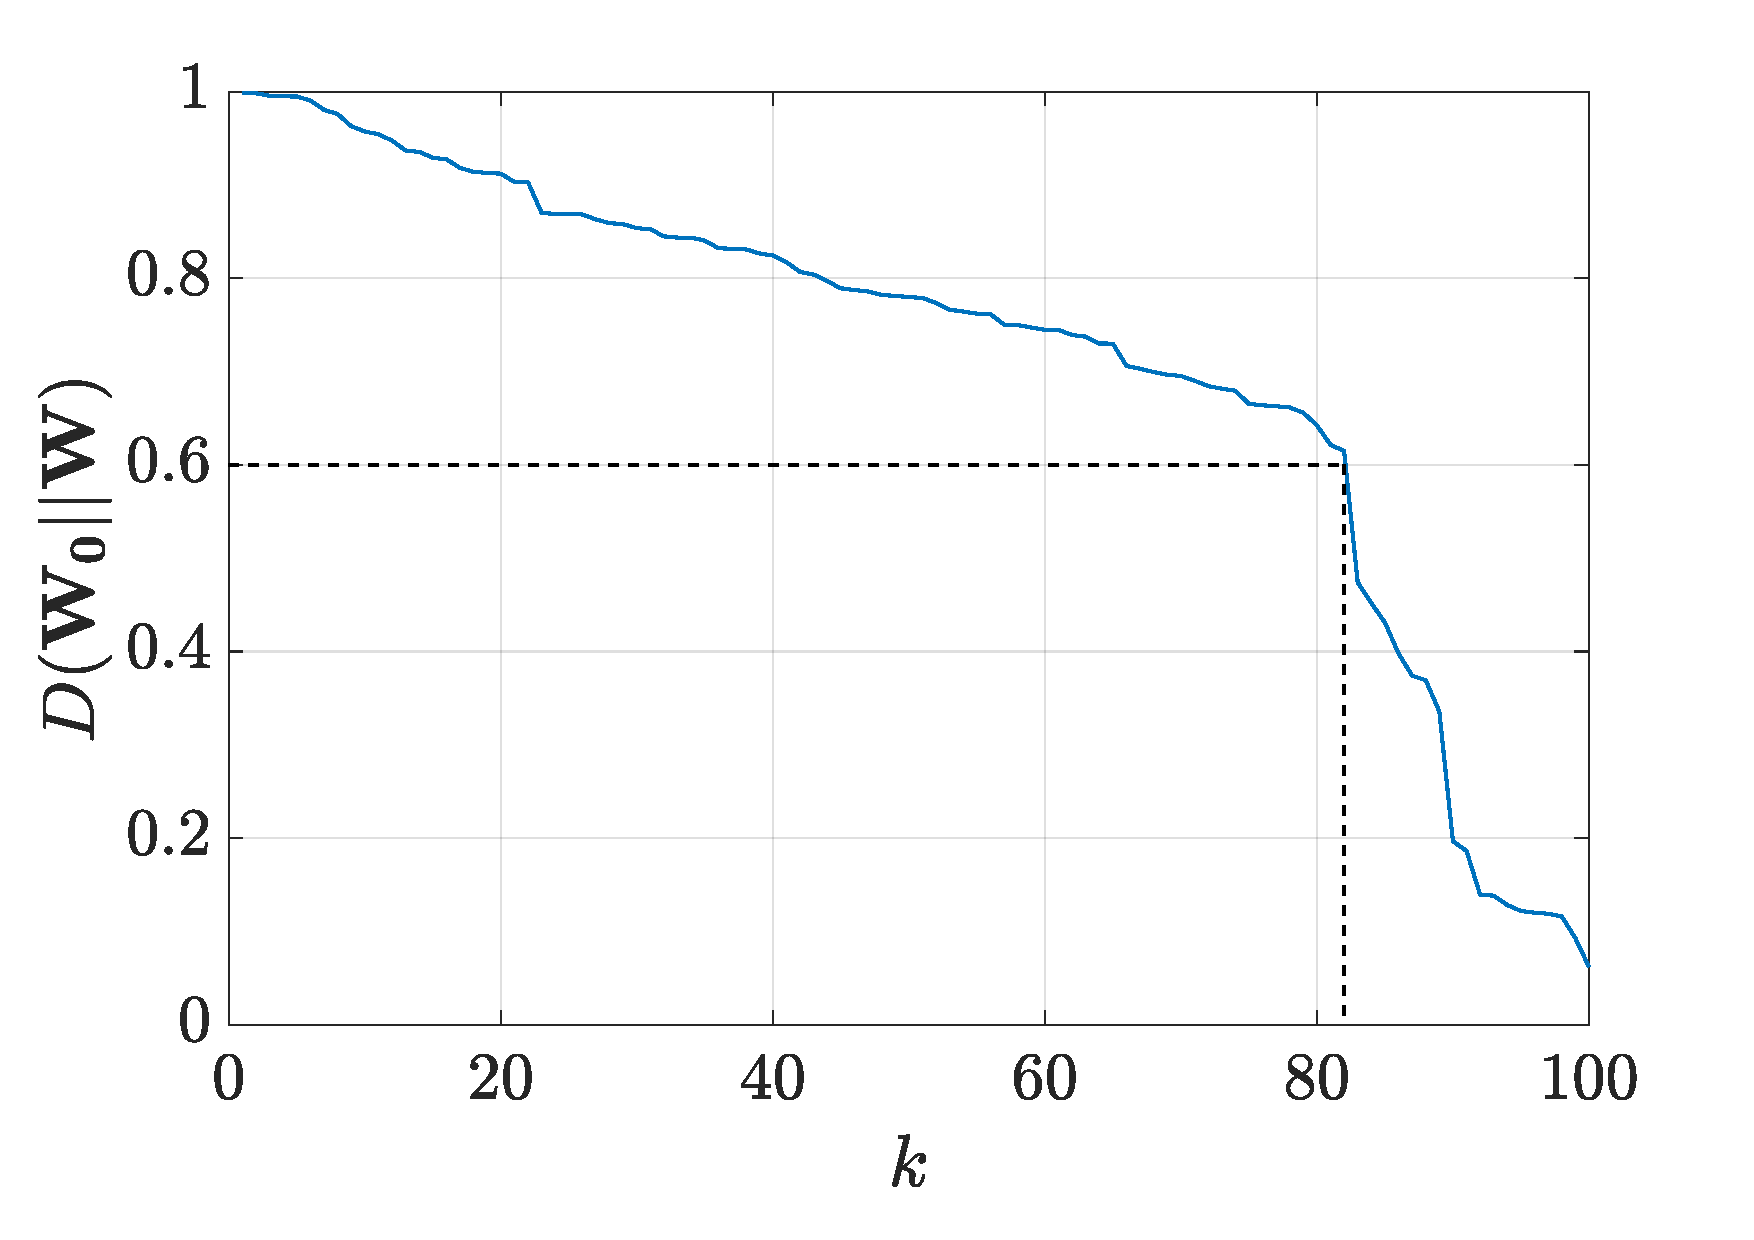
\includegraphics[width=0.8\linewidth]{figures/distanceCosLinDisplay.pdf}
\caption{Example of the $\mathbf{W}_{traffic}$ extraction from the sorted cosine similarity with a threshold $t = 0.6$. The $82$-nd first elements are considered as traffic component.}
\label{fig:W_ThC_NMF}
\end{figure}

This approach is named \textit{Thresholded inititialized NMF}, TI-NMF. Other thresholding methods as the \textit{soft} \cite{donoho1995noising}and the \textit{firm} \cite{fornasier2008iterative} and multiples way to display the distance through a sigmoïd or a Radial Basis Function have been investigated. A fast parametric study has revealed that the \textit{hard} thresholding method  with a linear representation of the similarity according to $K$, like in  Figure \ref{fig:W_ThC_NMF}), was the best way to get better performances.


\section{Experimental protocol}\label{part:protocol}

In order to validate the usefulness of considering NMF framework to estimate the road traffic noise level, one need to have a reference level. It can hardly be measured or even annotated from real life recordings. Thus,  simulated sound scenes are used to assess the performance of the proposed NMF. This offers a controlled framework to design specific sound environments in which all the traffic component is known. Then, the road traffic sound levels estimated with the method can be compared to the real ones, introduced within each simulated sound scene.

\subsection{Environmental sound scene corpus}

A corpus is designed with the \textit{simScene} software\footnote{Open-source project available at: \url{https://bitbucket.org/mlagrange/simscene}}. \textit{simScene} \cite{rossignol_simscene:_2015} is a simulator that creates sound scenes in a .wav format by summing audio samples that come from an isolated sound database.

This database is divided in two categories: $i)$ the \textit{event} category which are the brief sounds (from 1 to 20 seconds) that are considered as salient including 245 sound event samples divided in 19 sound classes (\textit{ringing bell, birds, sweeping broom, car horn, car passages, hammer, drill, coughing, barking dog, rolling suitcase, closing door, plane, siren, footstep, storm, street noise, train, tramway, truck and voice}) and $ii)$ the \textit{background} category that includes all the sounds that are of long duration and whose acoustic properties do not vary with respect to time. 154 sound samples belong to this category divided in 9 sound classes (\textit{birds, construction site noise, crowd, park, rain, children playing in schoolyard, constant traffic noise, ventilation, wind}). The sound class \textit{car passages} comes from 60 recordings of 2 cars made on the Ifsttar's runway on different speeds with multiple gear ratio. The other audio files have been found online (\textit{freesound.org}) and within the \textit{UrbanSound8k} database \cite{salamon_dataset_nodate}. Each sound classes is composed of multiples samples (\textit{bird01.wav}, \textit{bird02.wav} \dots).
The software allows the user to control some parameters (number of events of each class that appear in the mixture, elapsed time between each sample of a same class, presence of a fade in and a fade out \dots) completed with a standard deviation that may bring some random behavior between the scenes. Furthermore, an audio file of each sound class present in the scene can be generated that allows to know its exact contribution as well as a text file that summarizes the time presence of all the events.\\

\begin{figure}[t]
\centering
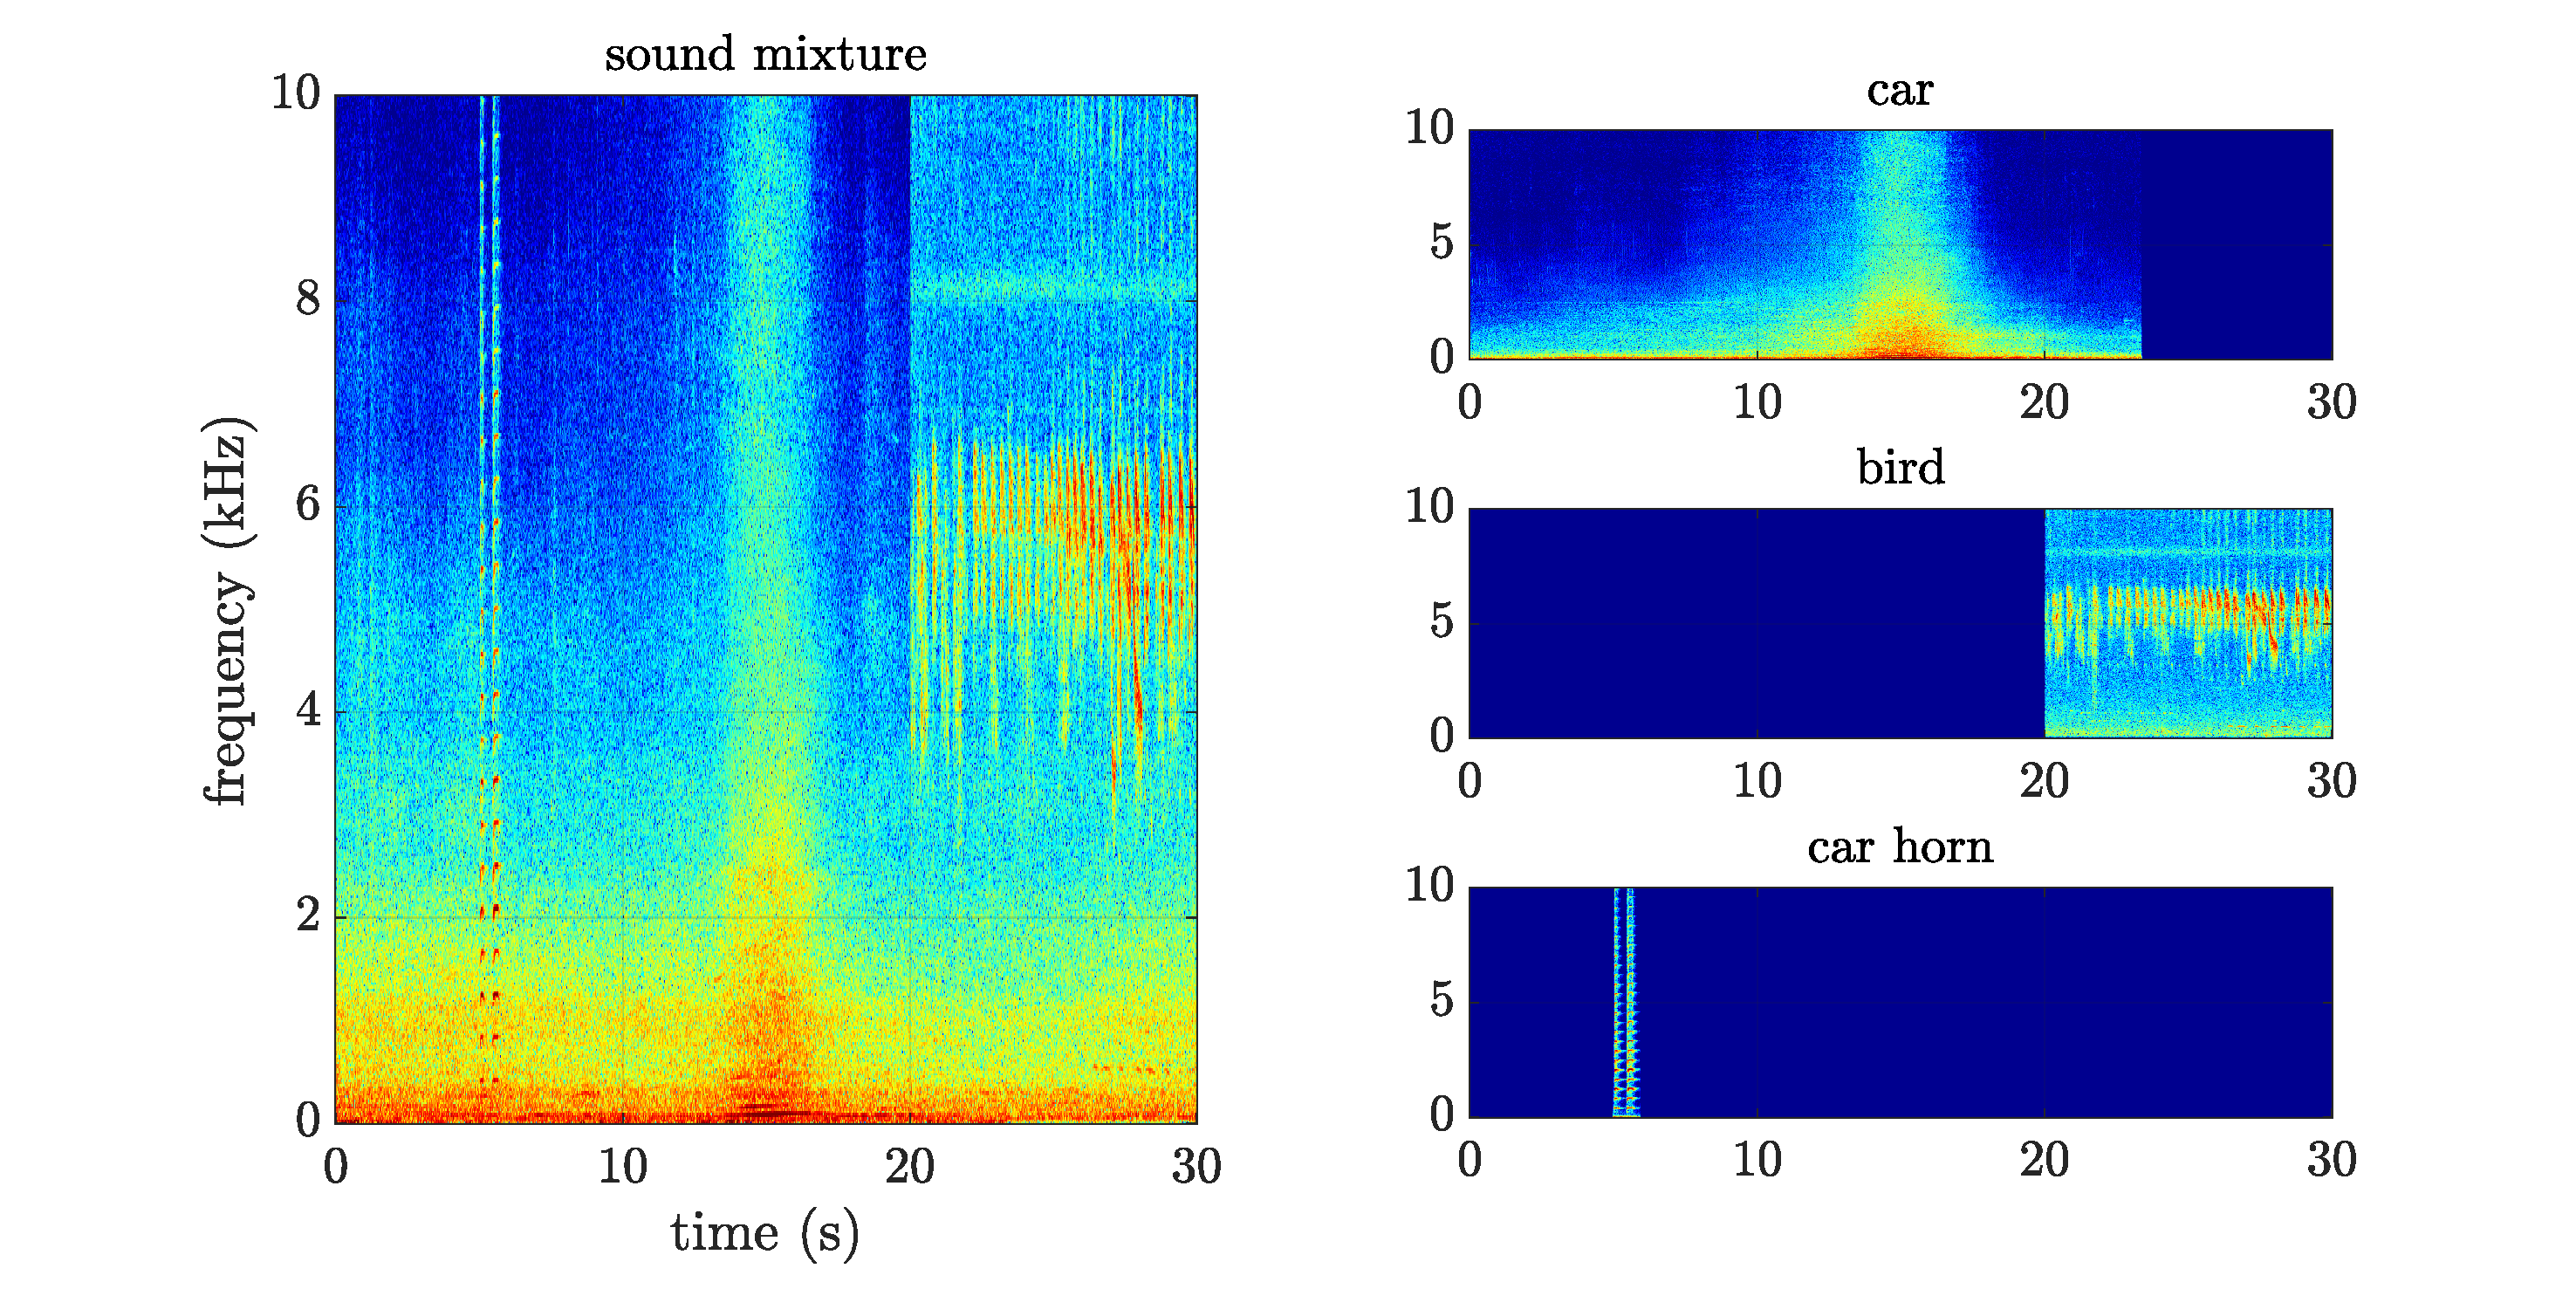
\includegraphics[width=\linewidth]{figures/exampleSimScene2.pdf}
\label{fig:exampleSimScene}
\caption{Example of a sound scene composed of 3 sound classes (car, bird, car horn)}
\end{figure}

This database enables creating realistic urban sound scenes from the road traffic point of view \cite{gloaguen_creation_2017}. A sound mixing corpus is composed of 6 sub-corpus of 25 audio files each lasting 30 seconds. Each sub-corpus is characterized by a specific generic sound class that summed with traffic will make the estimation of the traffic level more difficult. The classes are : \textit{alert} (car horn, siren), \textit{animals} (barking dog , whistling birds), \textit{climate} (wind, rain), \textit{humans} (crowd noise and voice), \textit{mechanics} (different metallic and construction site noises) and \textit{transportation} (train, tramway and plane). In each file, traffic component is present as the sum of the background and event traffic sounds and is mixed with the sound classes. The sound classes that are not related to the traffic component are summed up as the \textit{interfering} sound class. To test different scenarios, each audio file is duplicated with the traffic sound level of the entire sound scene, $L_{p,traffic}$, fixed to a specific level according to the sound level of the \textit{interfering} class, $L_{p,interfering}$ following the relation (\ref{eq:tir}).

\begin{equation}\label{eq:tir}
TIR = L_{p,traffic}-L_{p,interfering}
\end{equation}

with the \textit{Traffic Interference Ratio} $TIR = \left[-12, -6, 0, 6, 12\right]$. When $TIR = -12$, the traffic component is then less present than when $TIR = 12$ where it is predominant on the \textit{interfering} class. The 1 second equivalent sound pressure level, $p_{1s,traffic}$, is also calculated ; see Figure \ref{fig:exampleScene}). The total number of scenes designed is 750 (6 sub-corpus $\times$ 25 scenes $\times$  5 TIR values).

\begin{figure*}
\centering
   \begin{minipage}[c]{.32\linewidth}
      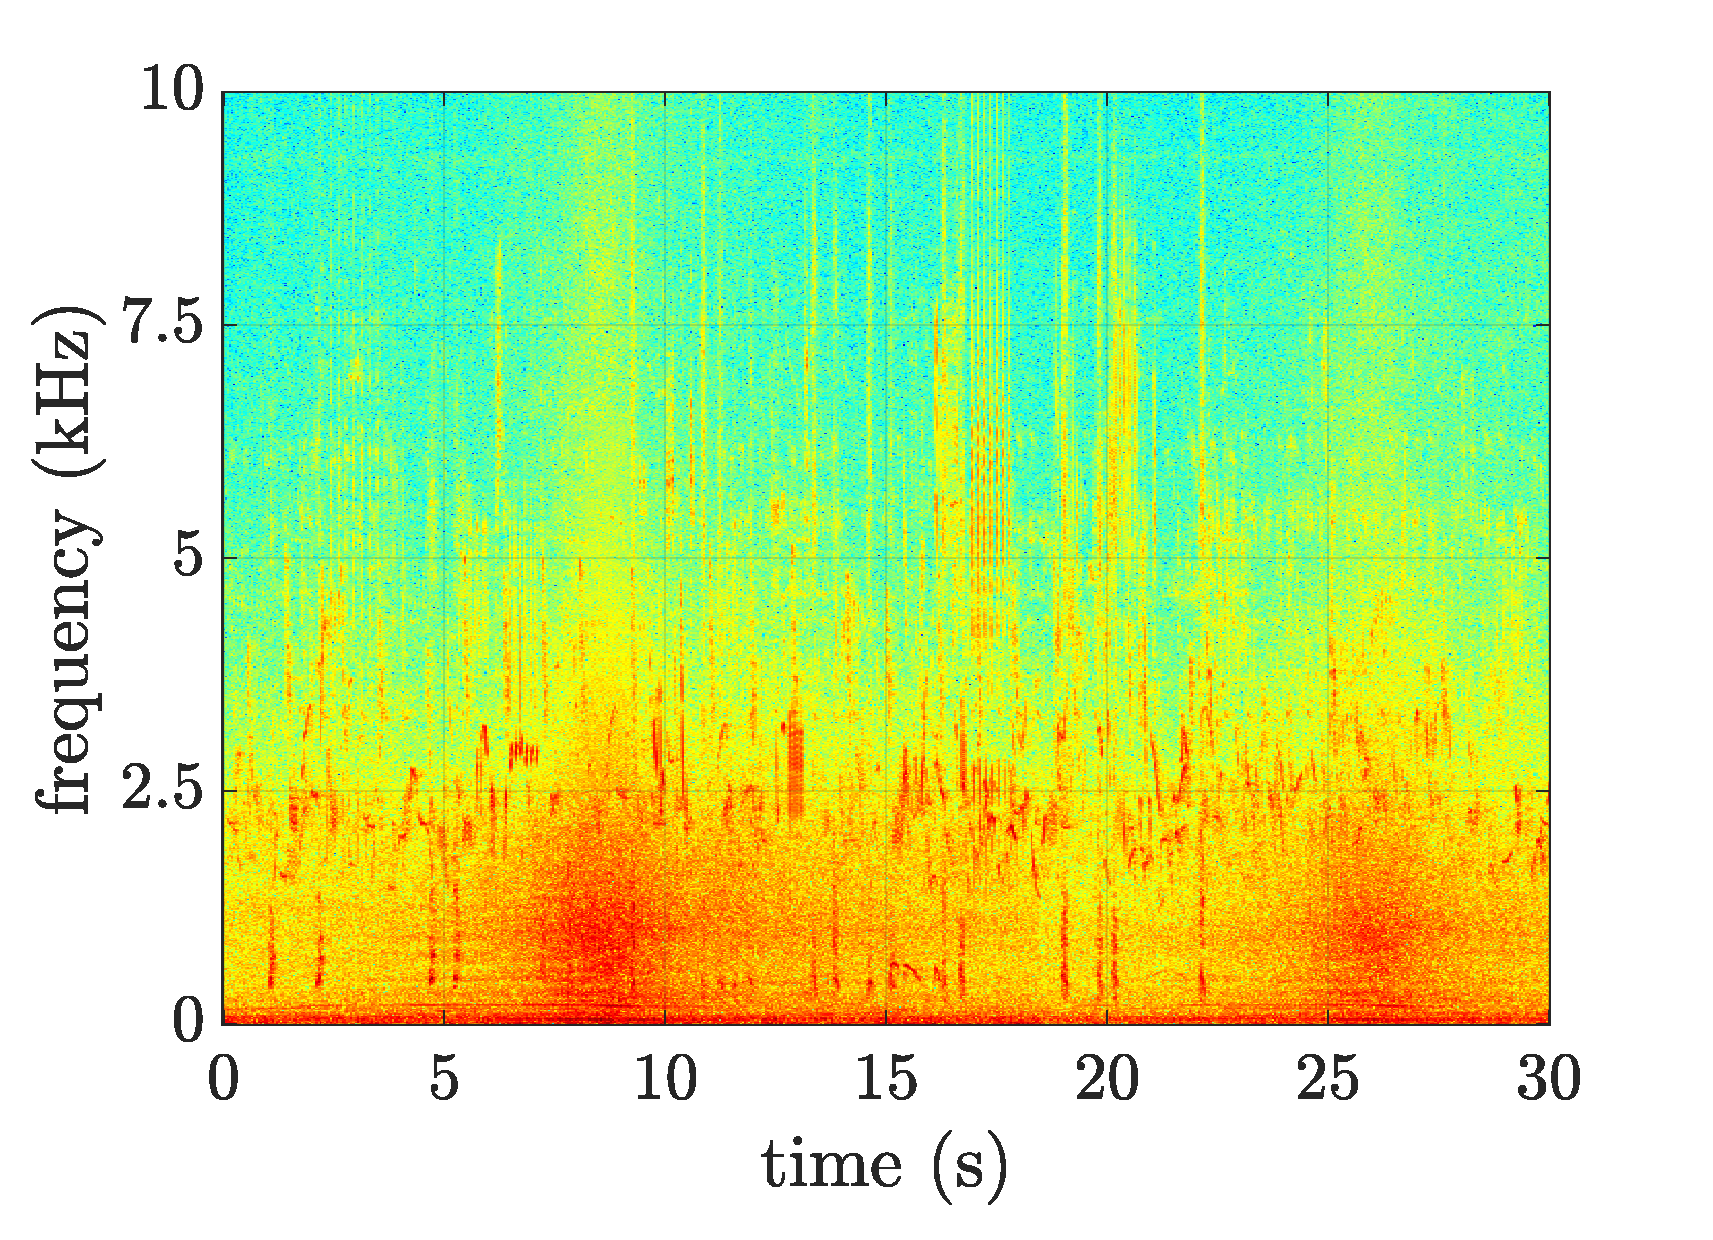
\includegraphics[width =\linewidth]{figures/spectrogramExample.pdf}
   \end{minipage}
   \begin{minipage}[c]{.32\linewidth}
      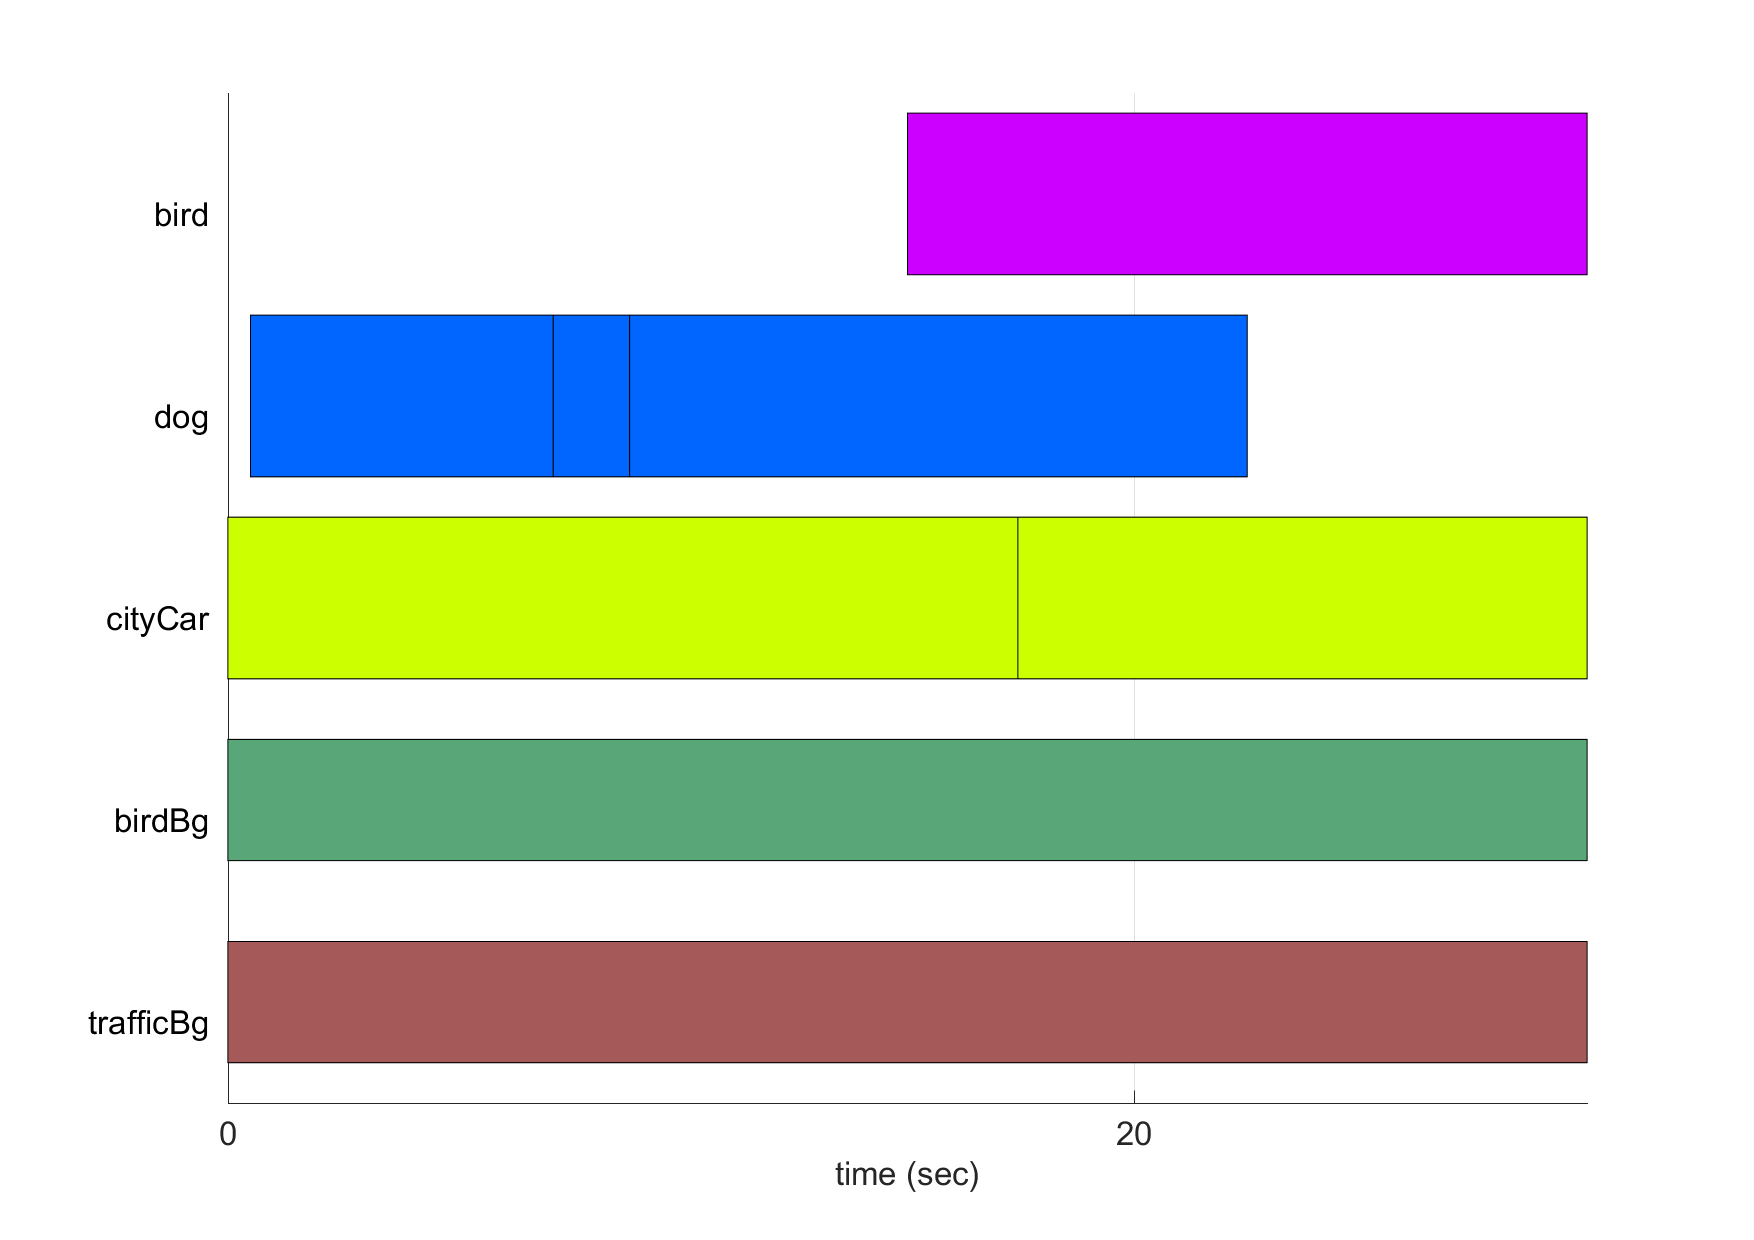
\includegraphics[width =\linewidth]{figures/animals_10-pianoRoll.png}
   \end{minipage}
   \begin{minipage}[c]{.32\linewidth}
      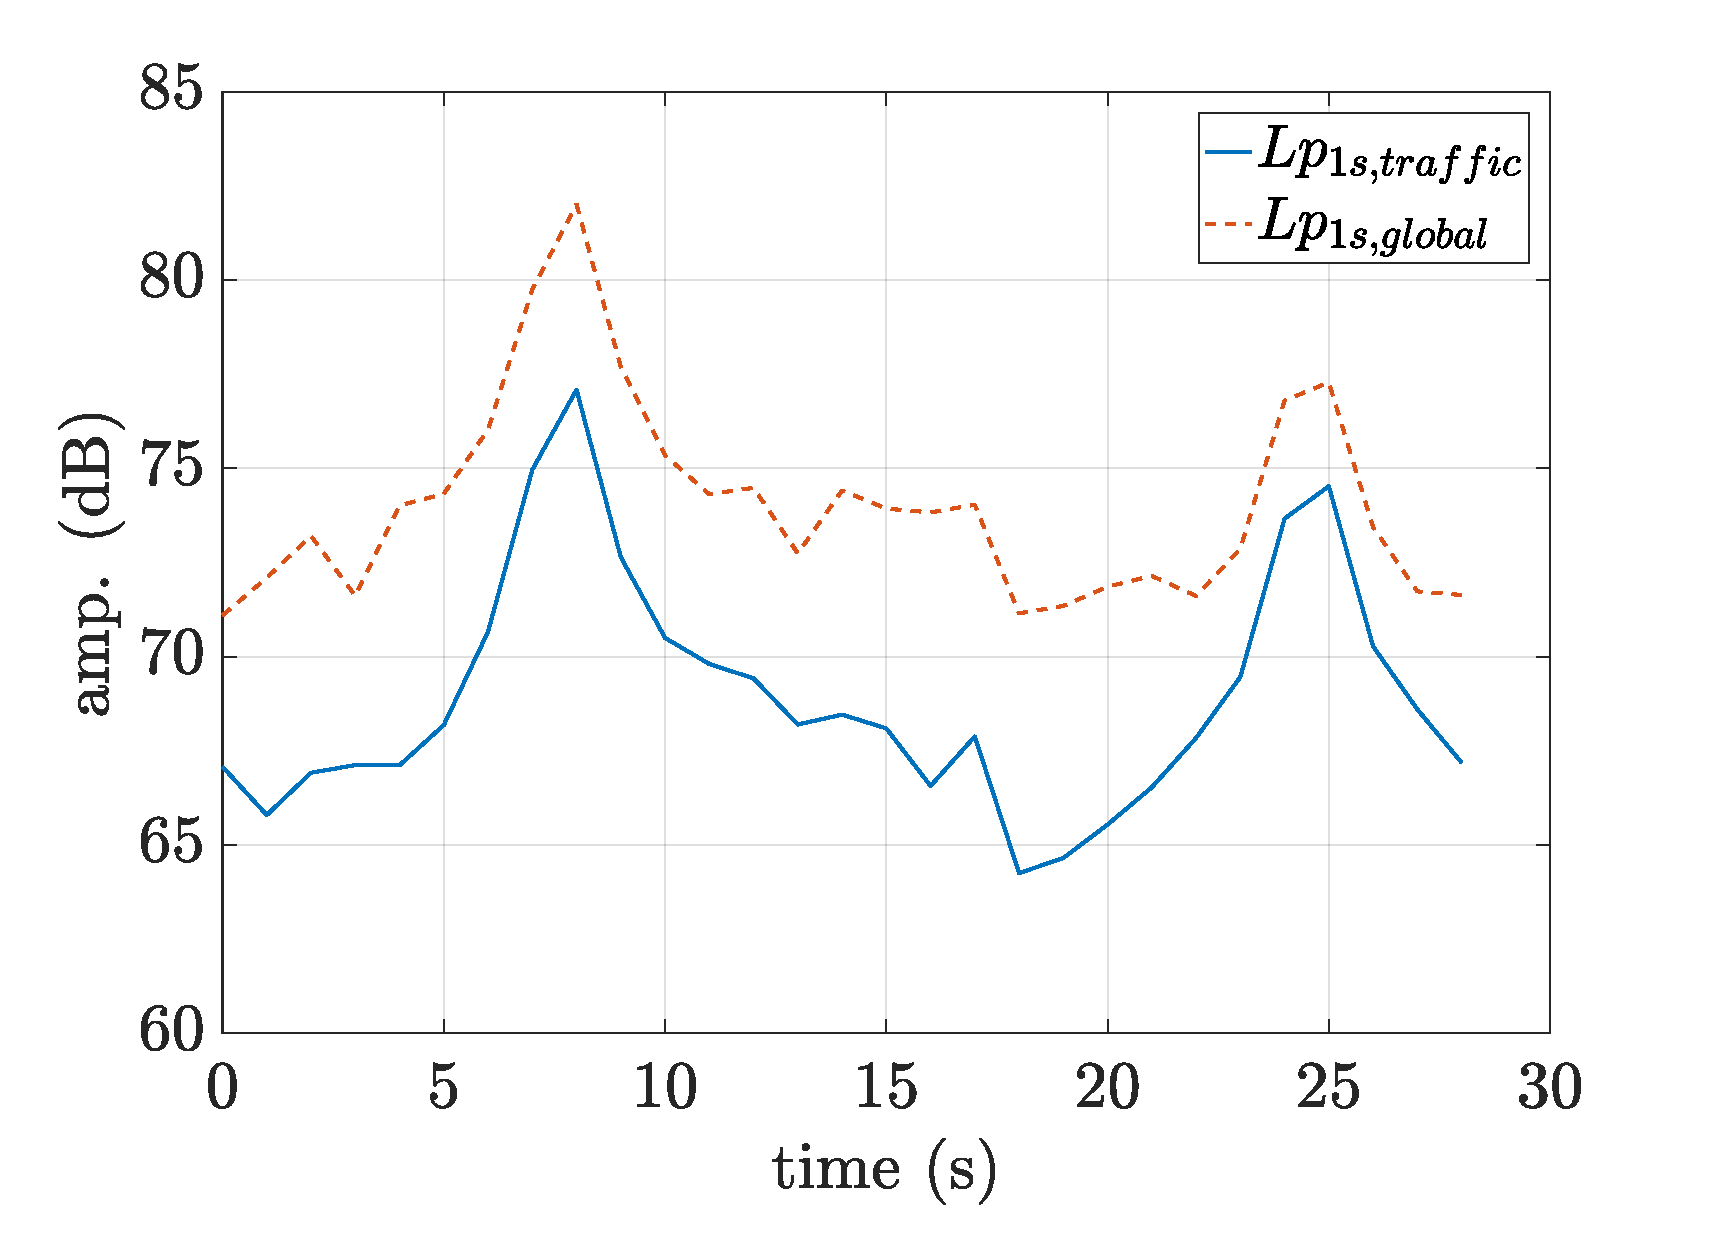
\includegraphics[width =\linewidth]{figures/evolutionLpExample.pdf}

   \end{minipage}
\caption{Example of a scene of the \textit{animals} sub corpus. Spectrogram (on left), \textit{Piano Roll} of the different sound classes (on the middle) and 1-s equivalent sound level of the traffic, $Lp_{1s,traffic}$ and of the global sound scene, $Lp_{1s,global}$(on right)}
\label{fig:exampleScene}
\end{figure*}

\subsection{Experiment}

The experiment consists in estimating the traffic road sound level of the 6 environmental sound sub-corpus (\textit{alert} (al), \textit{animals} (an), \textit{humans} (hu), \textit{climate} (cl), \textit{mechanics} (me), \textit{transportation} (tr)) and for 5 $TIR$ ([-12 -6 0 6 12] dB). First, the spectrogram $\mathbf{V}$ of each sound scene is built with a window size $w = 2^{12}$ with a 50 $\%$ overlap and a number of point $nfft = 2^{12}$. Therefore, the dimensions of $\mathbf{V}$ are $F$ = 2049 and $N$ = 664.

The first estimator to determine the traffic sound level is a frequency low-pass filter which depend only on the cut-off frequencies $f_c$ = [500 1k 2k 5k 10k 20k] Hz (see Figure \ref{fig:bloc_filtre}). The spectrograms $\mathbf{V}$ are filtered and the remaining energy is then considered as traffic component (eq. \ref{eq:v_tr_filtered}).

\begin{equation}\label{eq:v_tr_filtered}
\mathbf{\tilde{V}}_{traffic} = \mathbf{V}_{f_c}.
\end{equation}

The second estimator is the proposed scheme, based on several flavors of the NMF framework. Multiples experimental factors are involved here between the dictionary learning and NMF (see bloc diagram in Figure \ref{fig:bloc_nmf}).

\begin{figure}

    \centering
    \begin{subfigure}[t]{0.45\textwidth}
        \centering
        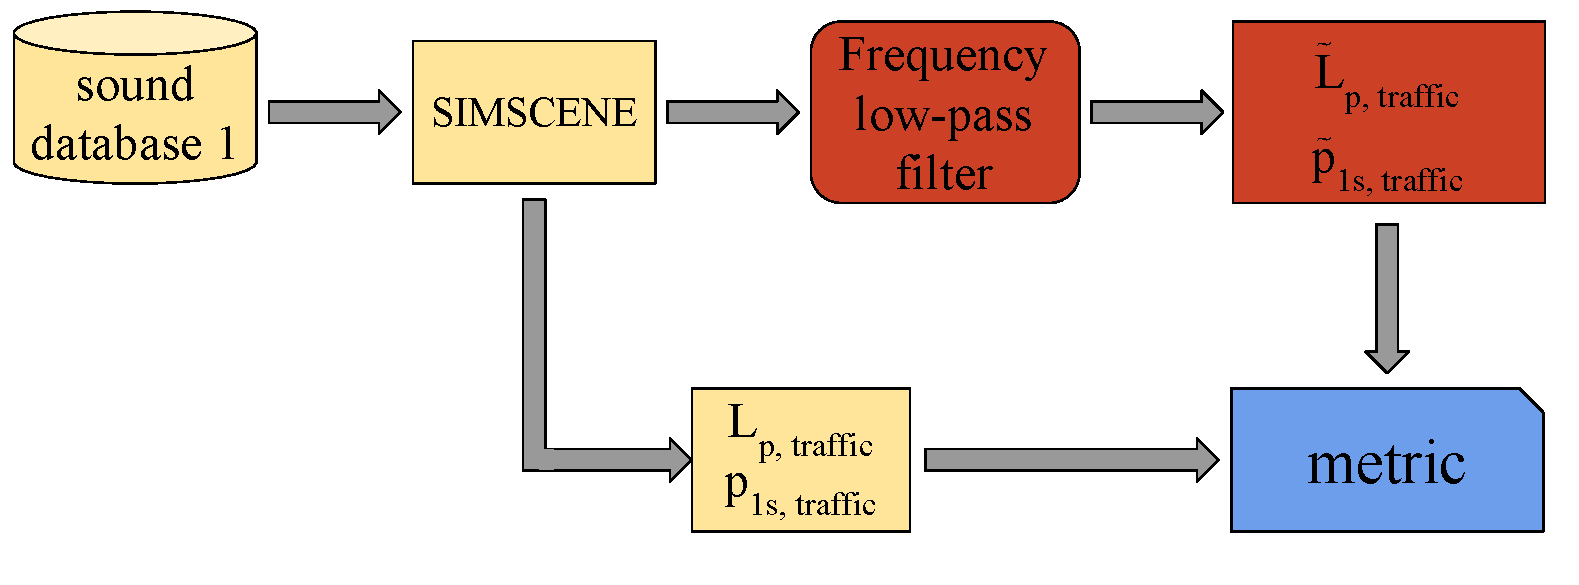
\includegraphics[width=\linewidth]{figures/bloc_diagram_filtrage_EN.pdf}
  		\caption{}
  		\label{fig:bloc_filtre}
    \end{subfigure}%
    \vfill
    \begin{subfigure}[t]{0.45\textwidth}
        \centering
        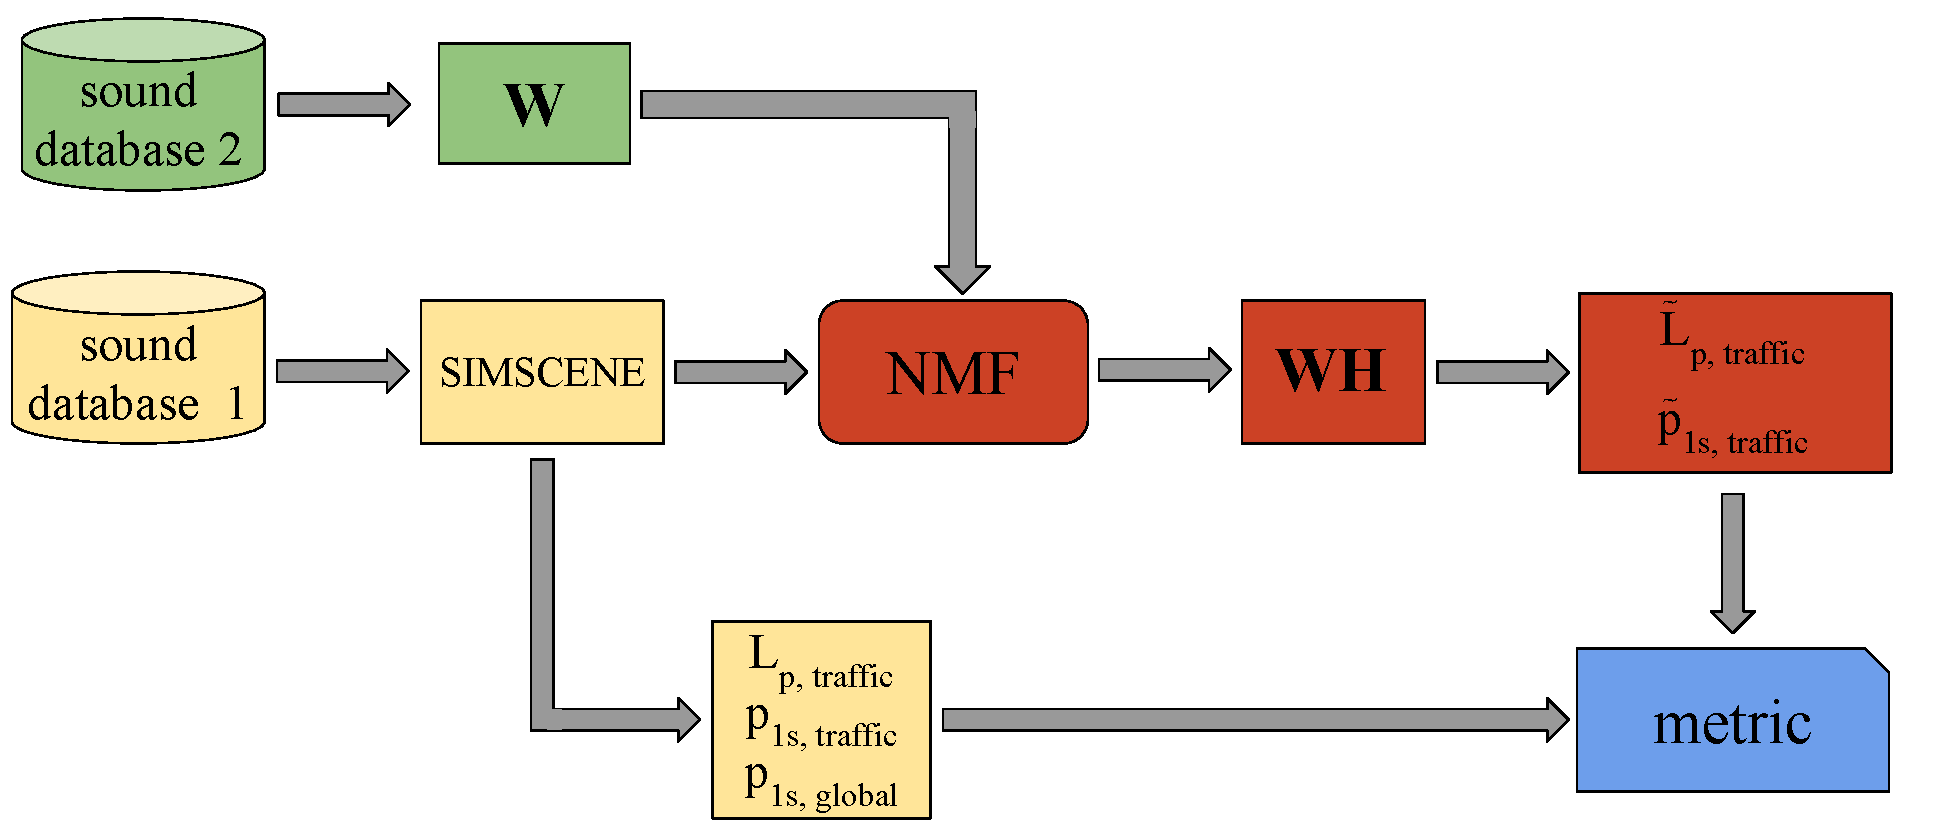
\includegraphics[width=\linewidth]{figures/bloc_diagram_NMF_EN.pdf}
		\caption{}
		\label{fig:bloc_nmf}
    \end{subfigure}
    
    \caption{Block diagrams summed up the different step of the process for the frequency low-pass filter (a) and for NMF (b)}
\end{figure}

\subsubsection{Dictionary building}\label{part:dictionary_learning}

The dictionary is built from a second sound database dedicated specifically to this task. It is composed of 53 audio files of passing cars. These records have been made on the Ifsttar's runway with the same conditions that the records made for the \textit{SimScene} database but with two different cars. First, for each audio file, its spectrogram is calculated with fixed parameters ($w$, 50 $\%$ overlap, $nfft$). Then time/frequency windows with $w_t \times F$ dimension are applied without overlapping on the spectrogram in order to consider several spectrum for each audio file. $w_t$ is fixed at $wt = [0.5 1]$ second. In each window, the root mean square value is calculated on each frequency bin to reduce the different spectrum in one spectra. Since the number of elements given by processing all the sound database is high, in order to reduce the computational and delete redundant information, a $K$-means clustering is applied to reduce the number of spectrum to $K = \left[ 25, 50, 100 \right]$. A special case is added where the root mean square of \textit{all} the spectrogram is applied. Each audio file generates one element $k$ of $\mathbf{W}$. An example that illustrates the process can be found on figure \ref{fig:dictionaryExtraction} on 3 seconds extract of a spectrogram of a car passage ; see Figure \ref{fig:specW}. In the case where $w_t$ = 1 second , 3 elements are therefore extracted of the spectrogram while in the case where $w_t$ = \textit{all}, all the spectrogram is reduced to one element ; see Figure \ref{fig:ElementW}.


\begin{figure}[t!]
    \centering
    \begin{subfigure}[t]{0.47\linewidth}
        \centering
       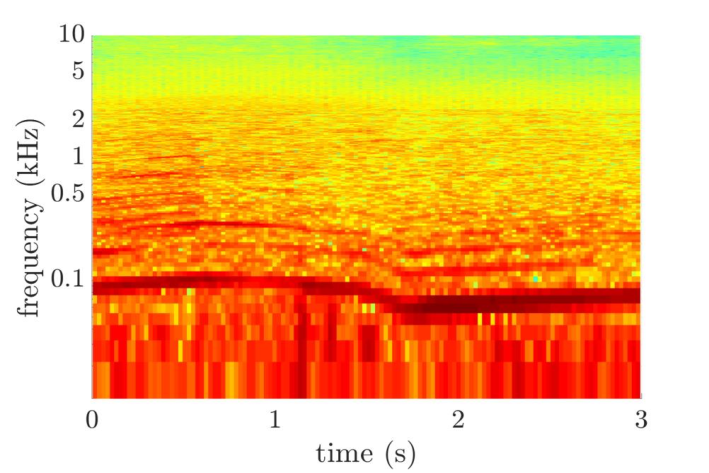
\includegraphics[width=\linewidth]{figures/dictionary1.pdf}
        \caption{Sample of 3 seconds of a car passage}
        \label{fig:specW}
    \end{subfigure}%
    \hfill
    \begin{subfigure}[t]{0.47\linewidth}
        \centering
       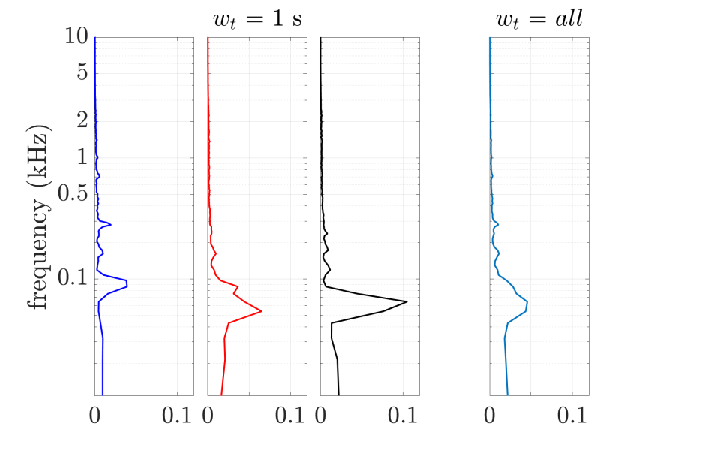
\includegraphics[width=\linewidth]{figures/dictionary2.pdf}
        \caption{Elements of the dictionary got for $w_t = 1$ second (3 spectrum) and  for $w_t = all$ (1 spectra) }
        \label{fig:ElementW}
    \end{subfigure}
\end{figure}


Each $k$ element of $\mathbf{W}$ is normalized such as $\vert \vert \mathbf{W_k} \vert \vert = 1$ with $\vert \vert \bullet \vert\vert$ the $\ell$-1 norm.\\

Table \ref{tab:dictionary_factors} summarizes the experimental factors and their related values.

\begin{table}[h]
\centering
\begin{tabular}{cccc}
Parameter &  \multicolumn{3}{c}{value}\\ \hline
$K$ & 25  & 50 & 100 \\ \hline
$\mathbf{w_t}$ (s)& 0.5 & 1  & \textit{all}
\end{tabular}
\caption{Summary of experimental factors of the dictionary}
\label{tab:dictionary_factors}
\end{table}

\subsubsection{Experimental factors of the NMF}

Supervised and semi-supervised NMF are performed for 400 iterations which is sufficiently enough to get a stabilized reconstruction. ThC-NMF is performed on a lower number of iteration (60) to prevent $\mathbf{W}$ to not deviate too much from the initial dictionary. The spectrogram $\mathbf{V}$ and the dictionary $\mathbf{W}$ are expressed on two different spectral representations: with a linear frequency scale ($\Delta f \approx 10.8$ Hz) and with third octave bands (29 bands). These two methods are considered to compare a fine grain approach (the linear scale) with a coarser one (the third octave bands) as it reduces the number of frequency bins in the high frequencies where the traffic component is less present and generates less calculations. Furthermore, in the case of the linear frequency scale and for supervised and semi-supervised NMF, $\mathbf{V}$ and $\mathbf{W}$ are filtered at the frequencies $f_c$ in order to focused the reconstruction of the signal of the low frequency bins. Nevertheless, if NMF is performed with filtered elements ($\mathbf{V}_{f_c}$ and $\mathbf{W}_{f_c}$) to determine $\mathbf{H}_{f_c}$, the traffic signal reconstruction is done with the original dictionary $\mathbf{W}$, as

\begin{equation}
\mathbf{\tilde{V}}_{traffic} = \left[\mathbf{WH}_{f_c}\right]_{traffic}.
\end{equation}

With the third octave spectral representation, only the case $f_c = 20$ kHz is applied. For the TI-NMF, the threshold is define between 0.20 and 0.70 with a 0.01 step. Table \ref{tab:estimation_factors} summarizes the experimental factors and their related values.

\begin{table*}[]
\centering
\begin{tabular}{lcccccc}
\textbf{Experimental factors} &  \multicolumn{6}{c}{value}\\ \hline
$\mathbf{TIR}$ (dB) & -12 & -6 & 0 & 6 & 12 &  \\ \hline
\textbf{sub-classes} & alert & animals & climate & humans & transportation & mechanics \\ \hline
$\mathbf{\beta}$ & \multicolumn{3}{c}{1} & \multicolumn{3}{c}{2} \\ \hline
$\mathbf{f_c}$ (kHz) & 0.5 & 1 & 2 & 5 & 10 & 20 \\ \hline
\textbf{method} & \multicolumn{2}{c}{filter} & supervised NMF & semi-supervised NMF & TI-NMF \\ \hline
$\mathbf{t}$ & \multicolumn{6}{c}{0.20:0.01:0.70} \\ \hline
\end{tabular}
\caption{Summary of the different experimental factors taken into account in the frequency low-pass filter and NMF process and their values for the estimation of the traffic sound level}
\label{tab:estimation_factors}
\end{table*}


\subsubsection{Metrics}
The performances of the two estimators of the road traffic sound level are assessed through the calculation of one metric, the Mean Absolute Error ($MAE$). It expresses the quality of the long-term reconstruction of the signal. It consists in the average over the $N$ sound scenes of the absolute difference between the exact and estimated traffic sound level in dB,

\begin{equation}
MAE = \frac{\sum_{n = 1}^N\vert L^n_{p,traffic}-\tilde{L}^n_{p,traffic} \vert}{N}.
\end{equation}

In all, according Tables \ref{tab:dictionary_factors} and \ref{tab:estimation_factors}, 24540 settings are performed between the different form of the dictionary $\mathbf{W}$ (table \ref{tab:dictionary_factors}) and the multiple experimental factors taken into account by NMF:  for the filter estimator, between the $TIR$, the sub-classes and $f_c$, 180 settings are performed whereas for supervised and semi-supervised, 7560 associations of factors are made. For TI-NMF, 16800 combinations can be calculated.

\section{Results}\label{part:results}

Table \ref{tab:results} summarized, according to the 3 main factors (method, $\beta$ and spectral representation), the $MAE$ error averaged on all sub-classes and all $TIR$ (750 sound mixtures in all).\\

\begin{table*}[]
\centering
\begin{tabular}{@{}cccccc@{}}
\toprule
$\mathbf{K}$ & $\mathbf{w_t}$ (s) &  $\mathbf{\beta}$ & \textbf{method} & $\mathbf{t}$ & \textbf{$MAE$ (dB)} \\ \midrule
 &  &  & filter &  & 4.69 ($\pm$ 4.52) \\
 &  &  & filter &  & 2.89 ($\pm$ 2.84) \\ \hline \hline
50 & 0.5  & 1 & supervised NMF &  & 3.44 ($\pm$ 3.70) \\
50 & 0.5  & 2 & supervised NMF &  & 3.02 ($\pm$ 3.33) \\ \hline \hline
100 & 0.5 & 1 & semi-supervised NMF &  & 2.38 ($\pm$ 1.26) \\
100 & 0.5 & 2 & semi-supervised NMF &  & 2.43 ($\pm$ 1.43) \\ \hline \hline
100 & all & 1 & TI-NMF & 0.57 & 2.19 ($\pm$ 2.01) \\
100 & all & 2 & TI-NMF & 0.54 & \textbf{2.16 ($\pm$ 2.24)}\\ \bottomrule
\end{tabular}
\caption{Best results according to $\beta$, method and  spectral representation}
\label{tab:results}
\end{table*}


The two first lines show the error produced by the baseline filter. $f_c = 20 $ kHz is equivalent to consider all the sound mixtures without distinguishing the traffic from the others sound sources. Consequently, in low $TIR$ (-12 and -6), where traffic component is scarce, the error is more important than in high $TIR$ (6 and 12) where the traffic component is predominant. $f_c = 500$ Hz is the cut-off frequency with the lower mean error obtained. It is then the baseline that will be used to compare the performances of NMF. In low $TIR$, for \textit{alert} and \textit{animals}, sub-classes composed of higher frequencies, the filter is efficient as it suppress these frequency components whereas for the other sub-classes where low frequencies are present, the error is higher as the filter considers all the energy located in the pass-band and then do not dissociate the traffic element from the other sound sources. The sounds levels are then overestimate ; see Figure \ref{fig:alert_-12}. In opposite, in high $TIR$, a low-pass filter at $f_c$ = 500 Hz removes too much energy from the traffic which has the consequence to underestimate the sound levels ; see Figure \ref{fig:alert_12}.\\


\begin{figure*}[t]
    \centering
    \begin{subfigure}[t]{0.45\textwidth}
        \centering
        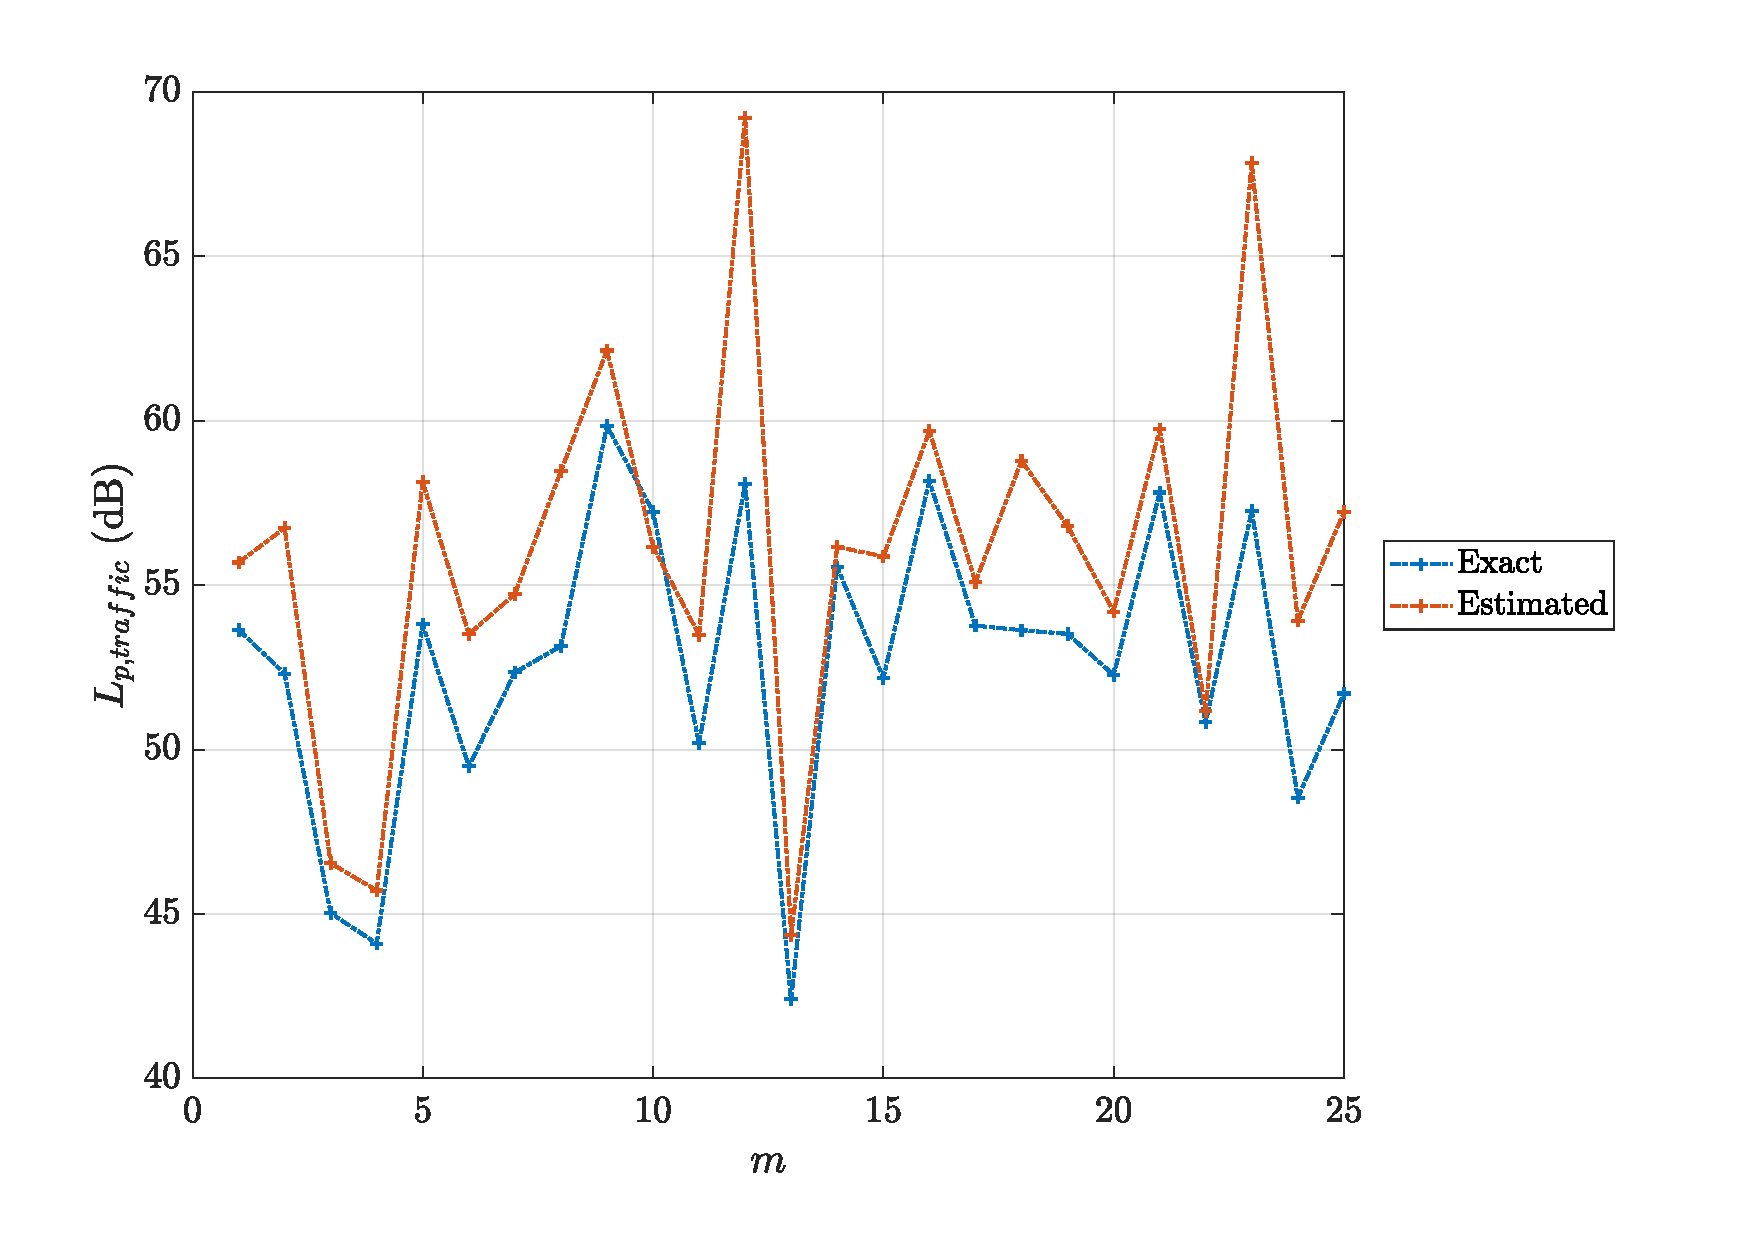
\includegraphics[width=\linewidth]{figures/LeqTrafficComparison_filter_alert_-12.pdf}
        \caption{}
        \label{fig:alert_-12}
    \end{subfigure}%
    \hfill
    \begin{subfigure}[t]{0.45\textwidth}
        \centering
        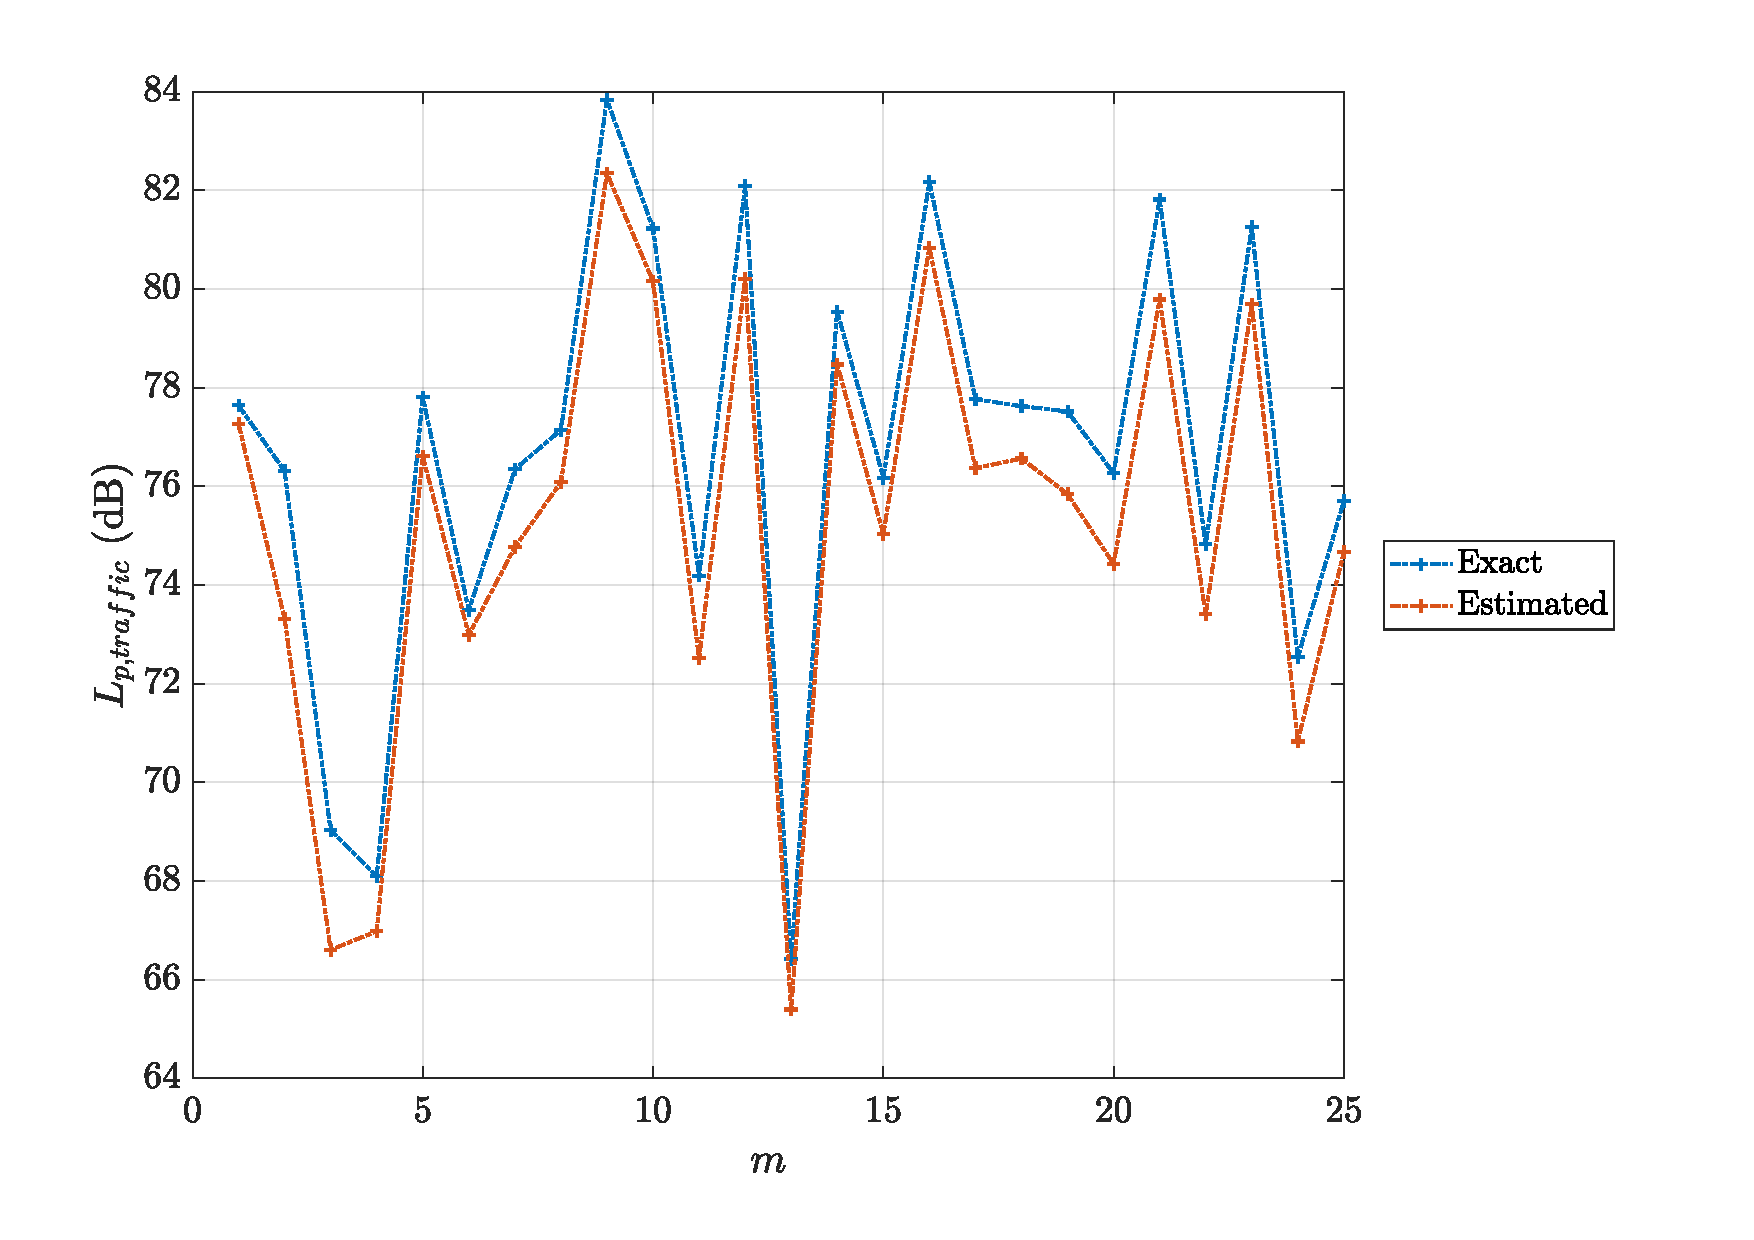
\includegraphics[width=\linewidth]{figures/LeqTrafficComparison_filter_alert_12.pdf}
        \caption{}
        \label{fig:alert_12}
    \end{subfigure}

    \caption{Global sound levels of the traffic estimated by the frequency low-pass filter with $f_c$ = 500 Hz for the sub-classes \textit{alert}: at $TIR = -12$ (\ref{fig:alert_-12}) and at $TIR$ (\ref{fig:alert_12}).}
    \label{fig:dictionaryExtraction}
\end{figure*}


The results of different versions of NMF are summarized next to the filter results in Table \ref{tab:results_TIR}. NMF errors lower than the baseline are put in bold letter. With the exception of supervised NMF with third octave spectral representation, all NMF have a lower mean error than the baseline. The best combination is got with a TI-NMF with a third octave spectral representation, $\beta$ = 2 and a threshold $t$ = 0.54.

Between the dictionary factors ($K$ and $w_t$) and the cut-off frequency $f_c$, none is common to all the settings. If for the third octave spectral representation, $f_c$ has been fixed at 20 kHz, in linear representation, this factors is variable depending on chosen method.

For supervised NMF, the spectrogram $\mathbf{V}$ has to be filtered at 500 Hz to focused the reconstruction of the signals on the part where most of the traffic energy is. According to the choice of $\beta$, the dictionary factors are different. It is the only case where it is.
In the opposite, in semi-supervised NMF, an unique set of factors is used to get high performance : $K$ = 100, $w_t$ = 0.5 second and $f_c$ = 20 kHz. It is with $f_c = 20$ kHz that the approximation is better as it includes easily other sound sources. With a lower cut-off frequency ($ f_c <$ 5 kHz), focusing on traffic energy, the risk is then to include \textit{traffic} component in $\mathbf{W_r}$ and to deteriorate the traffic signal reconstruction. The influence of the spectral representation and $\beta$ is here weak as the errors are similar with a low standard deviation. The third approaches, TI-NMF, proposed, in the four cases, the lowest errors. Like supervised NMF, in linear spectral representation, it is necessary to filter $\mathbf{V}$ to focus on the traffic energy. Here $f_c$ is higher (5000 Hz and 2000 Hz respectively for $\beta = 1$ and $\beta$ = 2). The choice of the spectral representation influence also the order of magnitude of the threshold $t$: in the interval [0.37 0.39] and [0.54 0.57] respectively for a linear and third octave spectral representation.\\

For each method (supervised, semi-supervised and TI-NMF), the best parameter combinations are detailed according to the sub-classes and the $TIR$ (Table \ref{tab:results_TIR},  Figure \ref{fig:TIR_class_filter}, \ref{fig:TIR_class_sup}, \ref{fig:TIR_class_semi} and \ref{fig:TIR_class_thc}). \\

\begin{table*}[t]
\centering
\begin{tabular}{@{}cccccc@{}}
\toprule
\textbf{method} & filter & filter & supervised NMF & semi-supervised NMF & TI-NMF \\ \midrule
$f_c$ (kHz) & 20 & 0.5 & 20 & 20 & 20 \\
$\mathbf{\beta}$ &  &  & 2 & 2 & 2 \\ \hline
\textbf{-12} & 12.25 ($\pm$ 0.05) & 7.36 ($\pm$ 3.00) & 6.23 ($\pm$ 3.19) &  & \textbf{5.11 ($\pm$ 3.10)} \\
\textbf{-6} & 6.96 ($\pm$ 0.05) & 3.44 ($\pm$ 1.65) & 3.00 ($\pm$ 1.39) &  & \textbf{2.87 ($\pm$ 1.55)} \\
\textbf{0} & 3.00 ($\pm$ 0.03) & 1.17 ($\pm$ 0.24) & \textbf{1.14 ($\pm$ 0.17)} &  & 1.38 ($\pm$ 0.38) \\
\textbf{6} & 0.97 ($\pm$ 0.01) & 1.03 ($\pm$ 0.26) & 1.01 ($\pm$ 0.28) &  & \textbf{0.70 ($\pm$ 0.32)} \\
\textbf{12} & 0.26 ($\pm$ 0.00) & 1.45 ($\pm$ 0.13) & 1.41 ($\pm$ 0.10) &  & \textbf{0.76 ($\pm$ 0.19)} \\ \bottomrule
\end{tabular}
\caption{$MAE$ error averaged on all sub-classes on each $TIR$ for the best scenario according to each method}
\label{tab:results_TIR}
\end{table*}


\begin{figure*}
    \centering
    \begin{subfigure}[t]{0.45\textwidth}
        \centering
        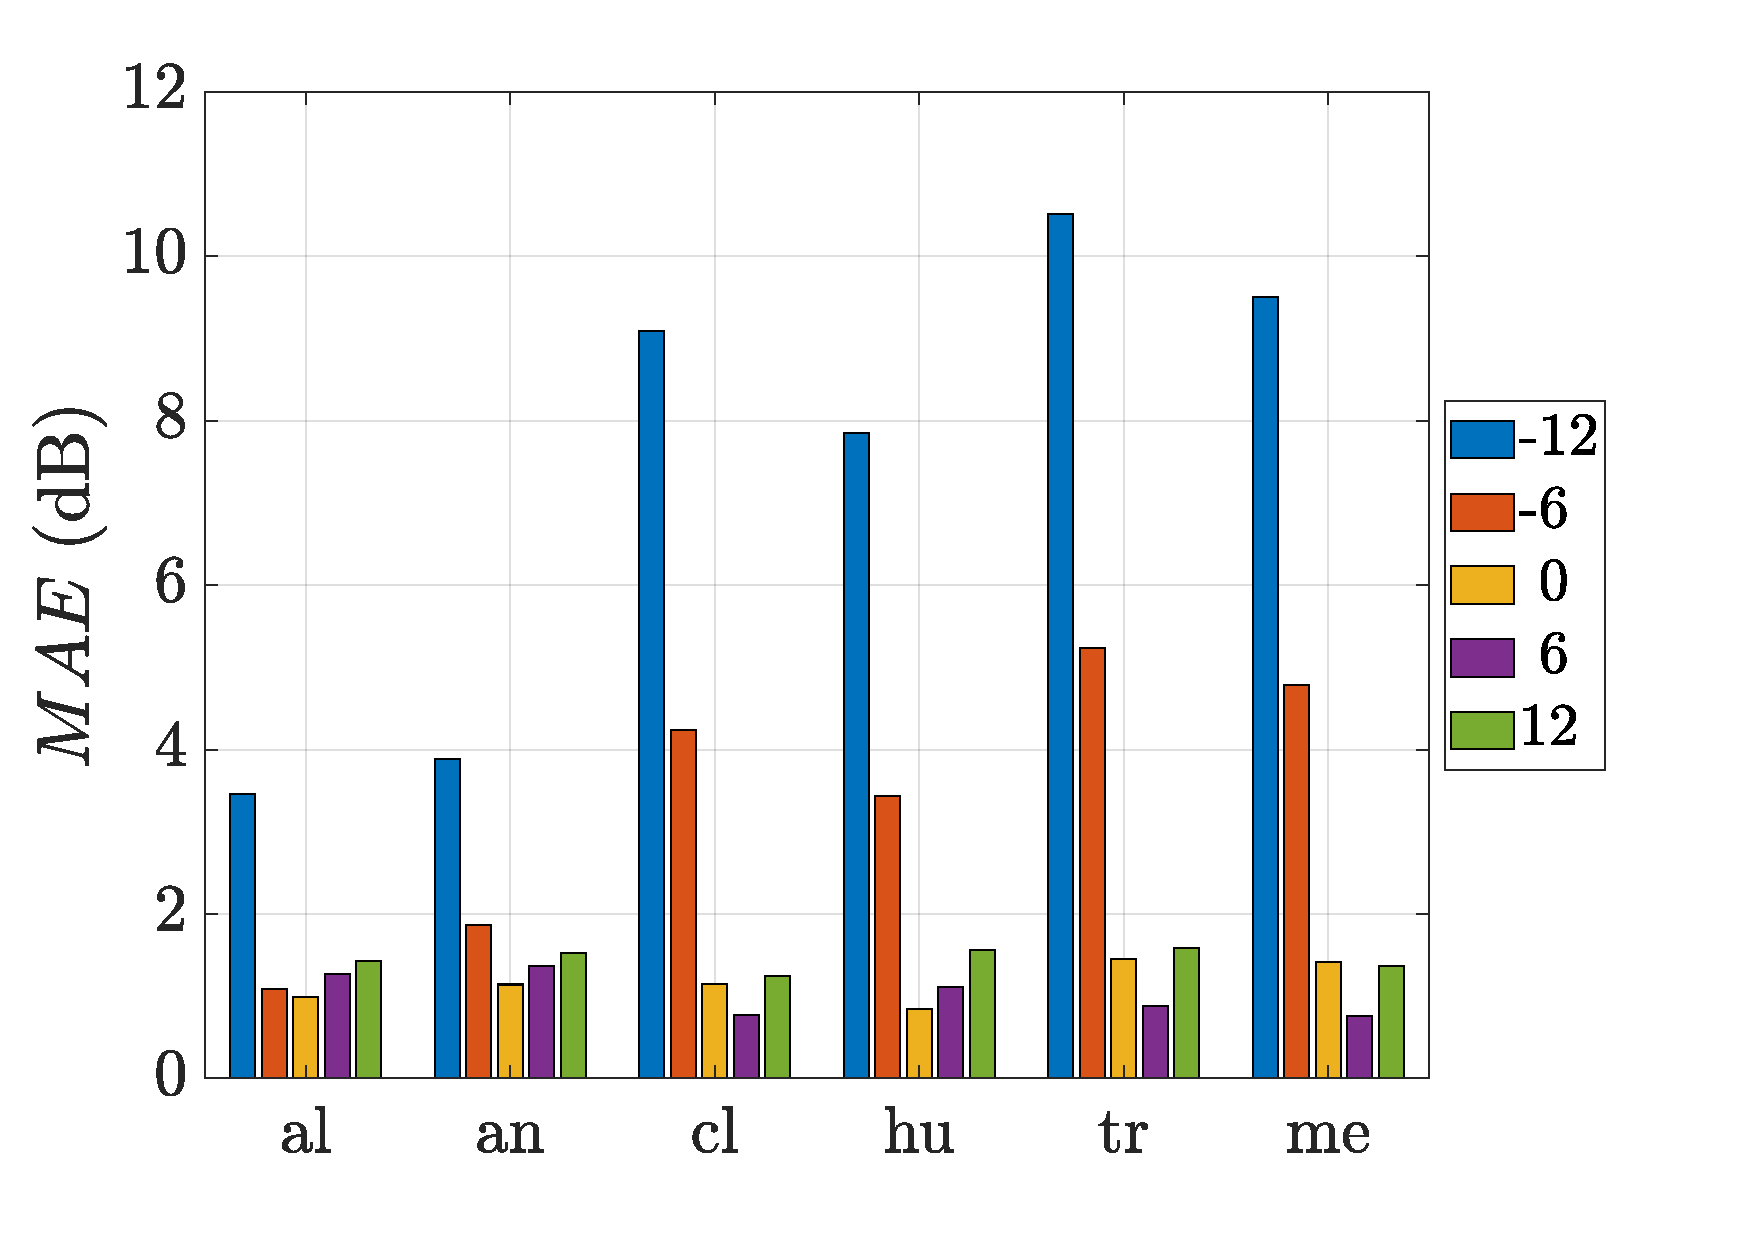
\includegraphics[width=\linewidth]{figures/filter_bar.pdf}
        \caption{Frequency low-pass filter with $f_c$ = 500 Hz}
        \label{fig:TIR_class_filter}
    \end{subfigure}%
    \hfill
    \begin{subfigure}[t]{0.45\textwidth}
        \centering
        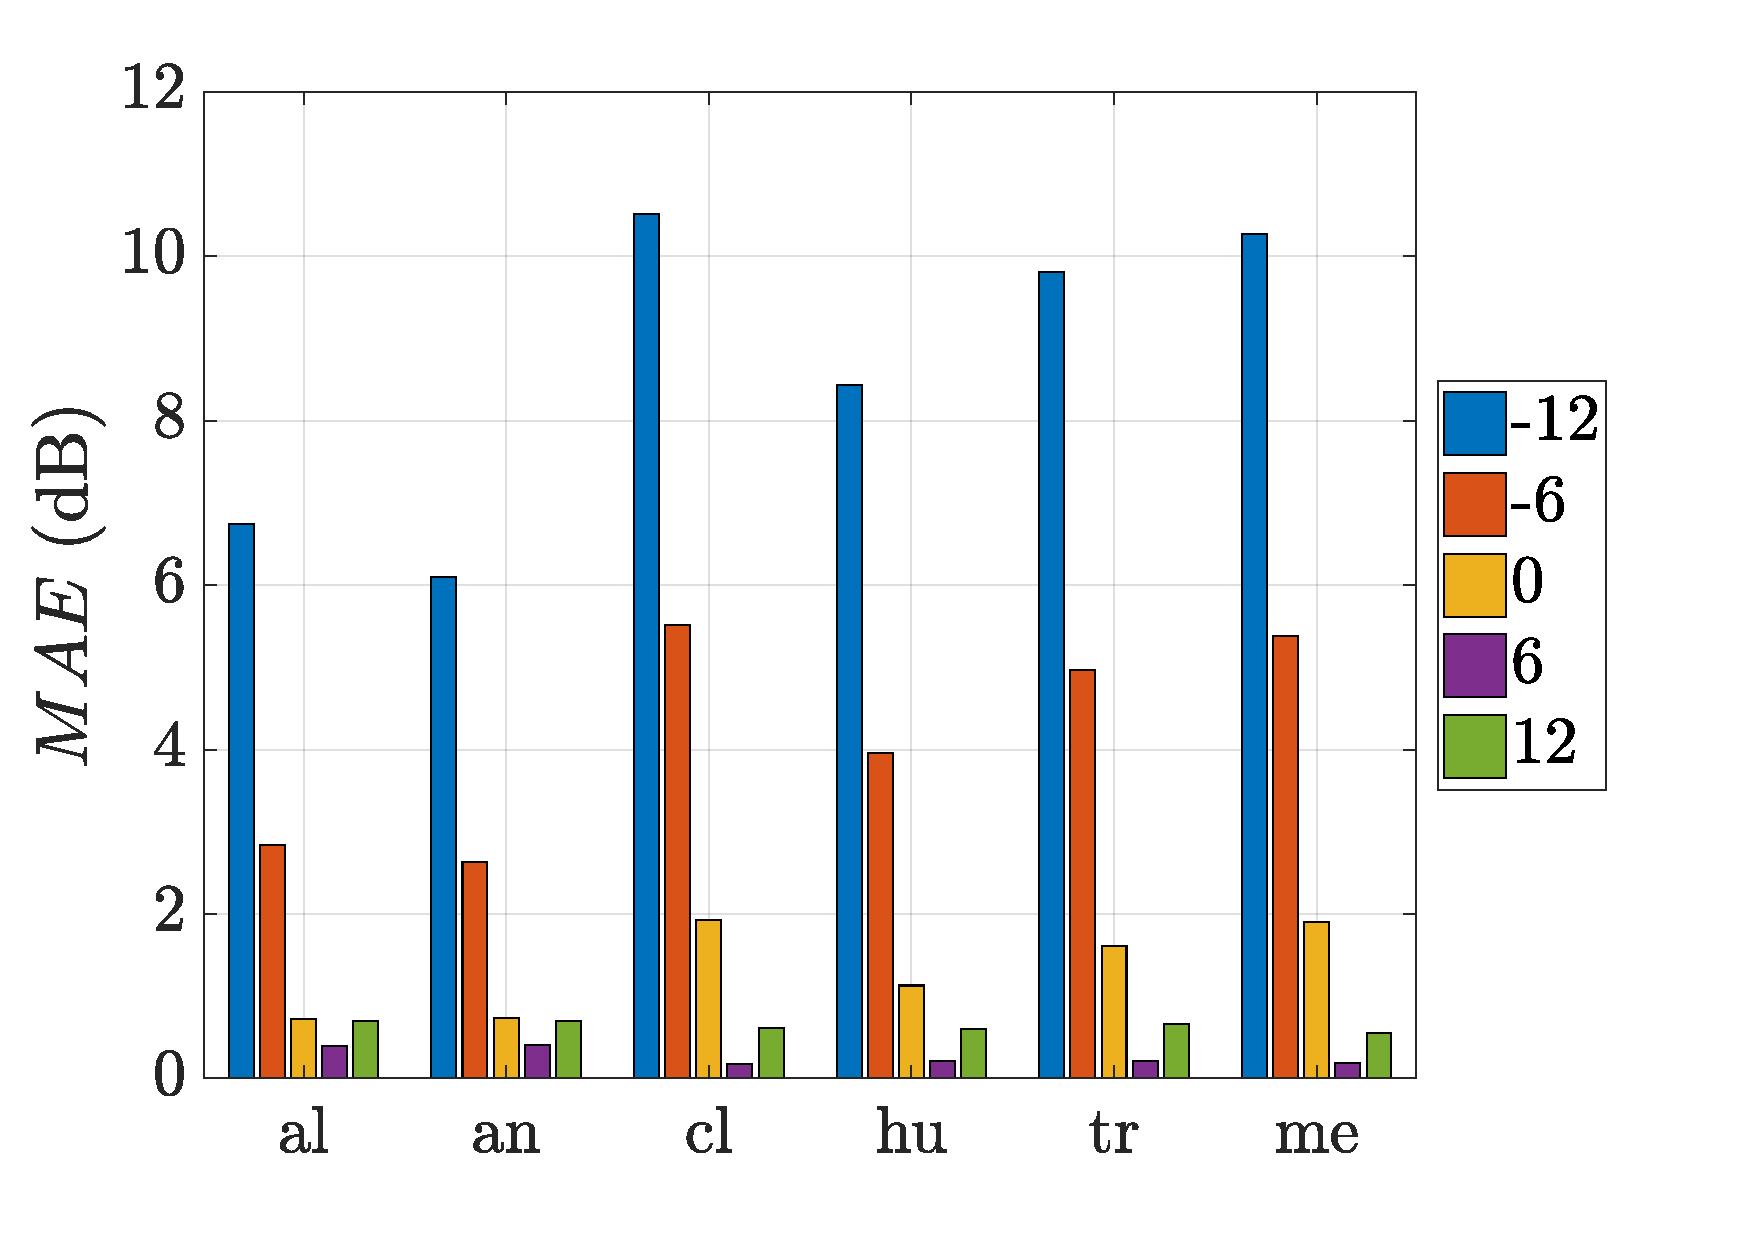
\includegraphics[width=\linewidth]{figures/sup_bar.pdf}
        \caption{Supervised NMF, $\beta$ = 2, linear spectral representation, $f_c$ = 0.5 kHz}
                \label{fig:TIR_class_sup}
    \end{subfigure}

    \begin{subfigure}[t]{0.45\textwidth}
        \centering
      	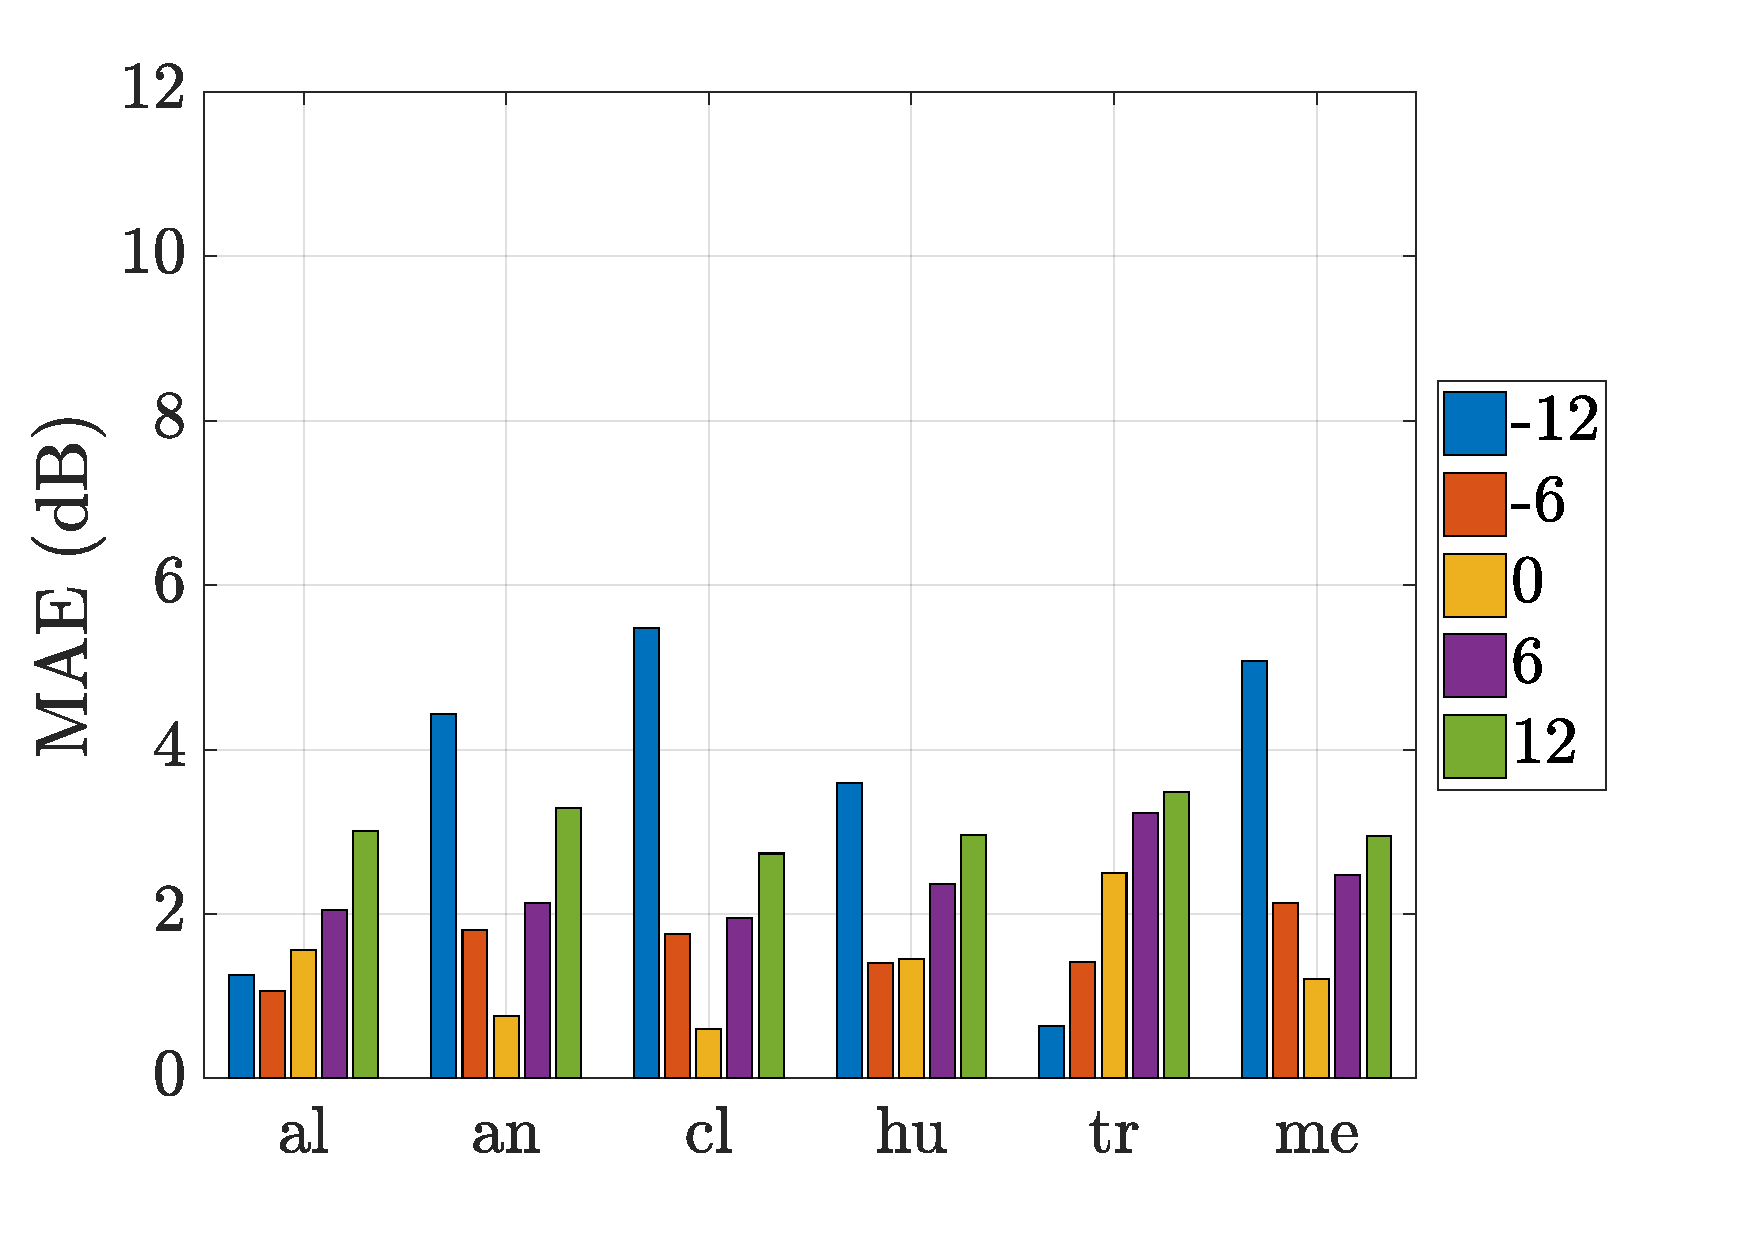
\includegraphics[width=\linewidth]{figures/semi-sup_bar.pdf}
        \caption{Semi-supervised NMF, $\beta$ = 2, linear spectral representation, $f_c$ = 20 kHz}
                \label{fig:TIR_class_semi}
    \end{subfigure}%
    \hfill
    \begin{subfigure}[t]{0.45\textwidth}
        \centering
        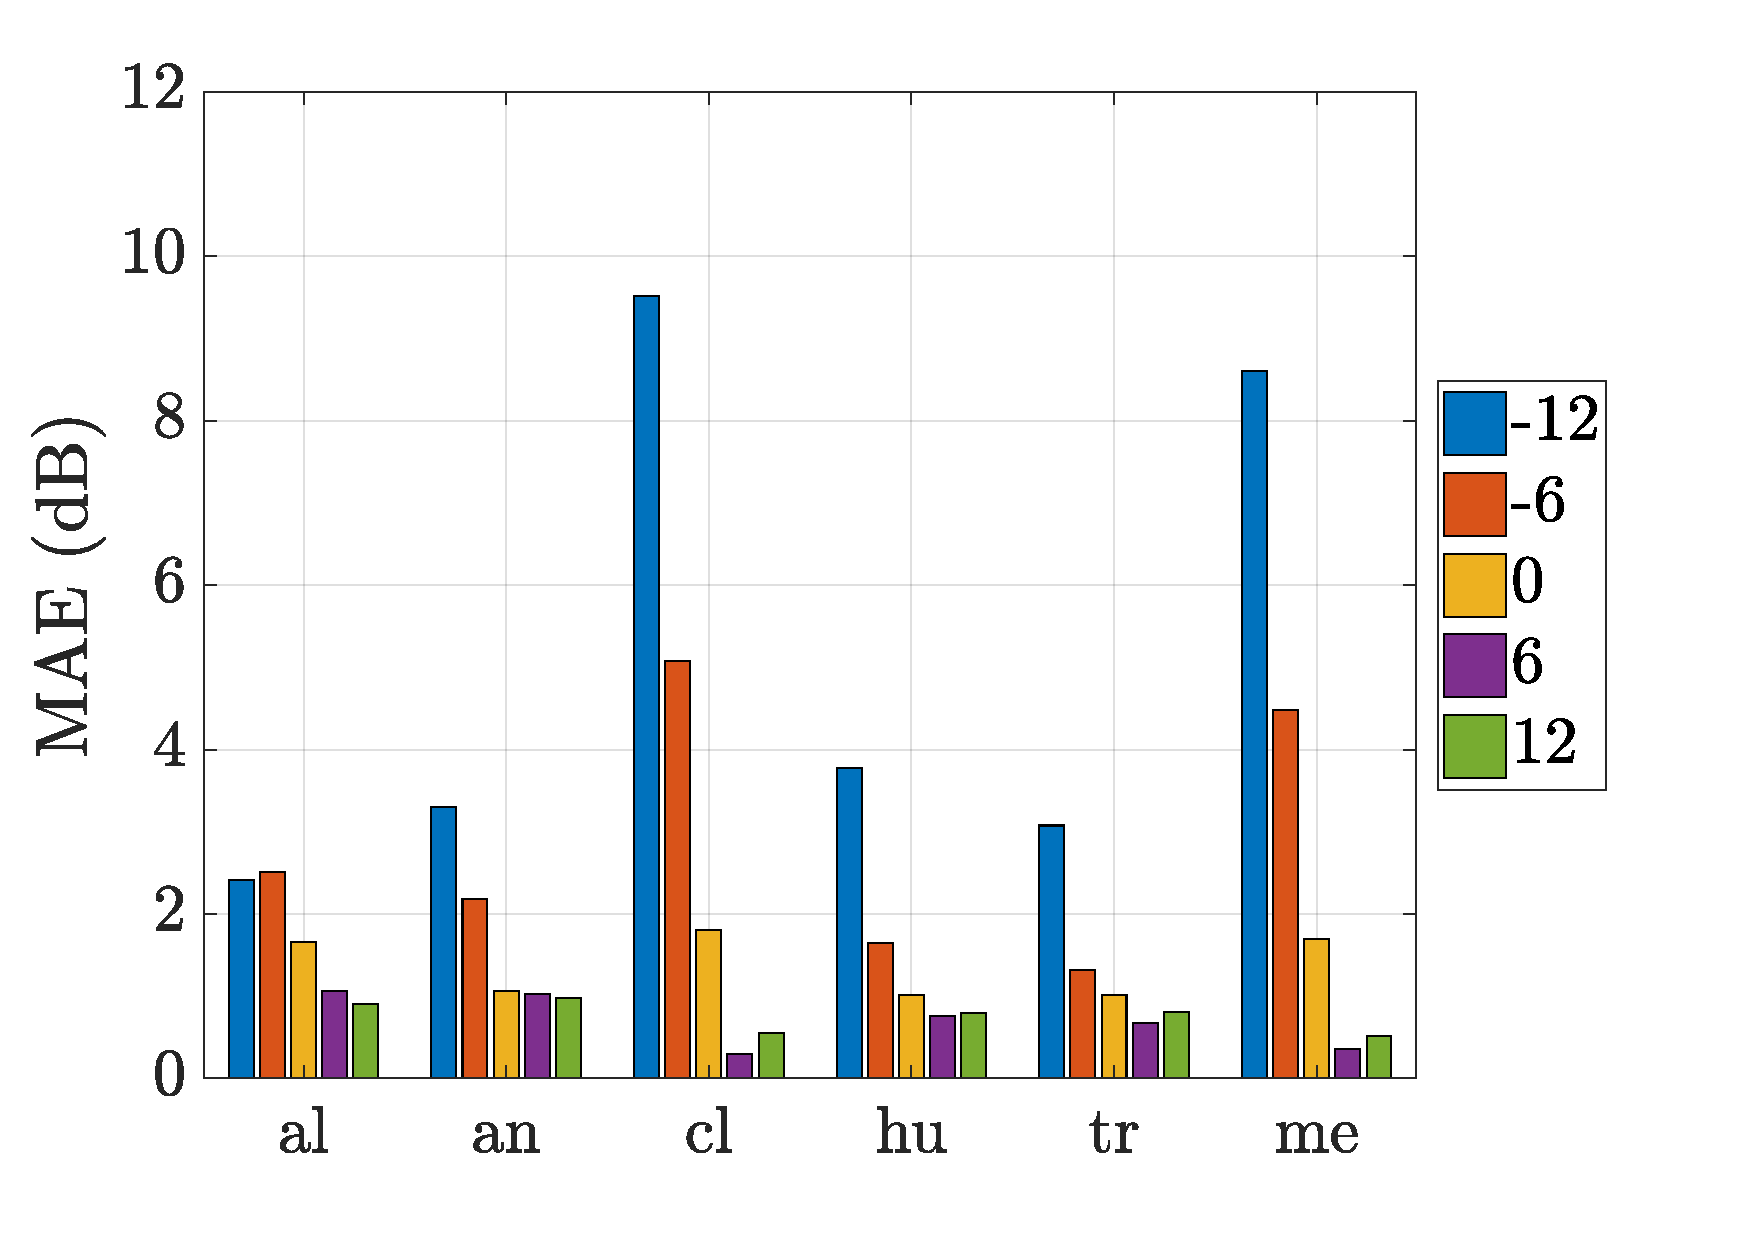
\includegraphics[width=\linewidth]{figures/THC_bar}
        \caption{TI-NMF, $\beta$ = 2, third octave spectral representation, $f_c$ = 20 kHz}
        \label{fig:TIR_class_thc}
    \end{subfigure}
    \caption{$MAE$ error for each sub-class and $TIR$ according to the the best results with the filter and each method (supervised, semi-supervised and ThC}
\end{figure*}

According to Figure \ref{fig:TIR_class_filter}, \textit{climate}, \textit{human}, \textit{transport} and \textit{mechanics} are the four sub-classes that generates the highest error levels particularly in low $TIR$ as they are sound classes composed of low frequency sound (storm for \textit{climate}, voices in \textit{humans}, plane in \textit{transport} and ventilation noise in \textit{mechanics}). All these kind of sounds are then considered as traffic component without distinction.
In the case of supervised NMF, on all the $TIR$, if the mean score on each $TIR$ is lower than the baseline method, it offers similar performances as for $TIR = [0, 6, 12]$, the mean scores are nearly close. The performance of supervised NMF is mainly visible for $TIR = -12$ where the error with the baseline decrease by more than 1 dB. This improvement is significant with the \textit{alert} sub-class as it gathers sounds that are mostly in higher frequencies ([2500 5000] Hz). From a dictionary $\mathbf{W}$ composed of traffic element, the traffic signal reconstruction is then easier. However, supervised NMF fails to improve significantly the baseline performances.

Meanwhile, semi-supervised approach with the add of a mobile part in the dictionary, $W_r$, brings a major improvement especially for the low $TIR$ as it can be see in Figure \ref{fig:TIR_class_semi}). By the add of $\mathbf{W_r}$, it allows to take into account the other predominant sound sources. An example can be found in Figure \ref{fig:Y_alert-12} which summarizes the obtained $\mathbf{W_r}$ of a scene belonging to \textit{alert} sub-class. The first element is mainly composed of harmonics signal which correspond to the car horn of the scene. The decreasing of errors can be seen on each sub class for $TIR = -12$ and $TIR$ = -6 in  where the error are much lower than supervised NMF.
As the $\mathbf{W}$ is only composed of \textit{traffic} element, this approach is likely to use traffic components to reduce it even if the sound source not traffic to reduce the distance/divergence between $\mathbf{V}$ and $\mathbf{WH}$ deteriorating the quality of traffic signal reconstruction.

The comparison can be made on a scene of the \textit{alert} sub-class:
FIGURE Lp 1 seconde avec supervisé et semi-supervisé pour voir l'utilisation des éléments trafic dans la supervisée et non dans al semi-supervisée. \\

However, the degrees of freedom of semi-supervised NMF are restrictive for high $TIR$ as the errors exceed 2 dB for all sub-classes. Indeed, in order to reduce the distance/divergence between $\mathbf{V}$ and $\mathbf{WH}$ without constraint semi-supervised NMF is free to include traffic components in $\mathbf{W_r}$. Consequently, this behaviors decreases the quality of the reconstruction of the traffic component. The same scene used in Figure \ref{fig:Y_alert-12}) but with $TIR$ can be seen in Figure \ref{fig:Y_alert_12} where the harmonic components of traffic have disappears for low frequency components. The error are then increasing for these $TIR$. Constrain $\mathbf{W_r}$ to avoid these behaviors and control what can be put into could be a way to improve this method here \cite{kitamura_music_2014}. In opposite, supervised NMF (that could be seen as semi-supervised NMF which is infinitely constrain on $\mathbf{W_r}$) offer a good reconstruction of the traffic signal from $\mathbf{W}$.\\

\begin{figure*}
    \centering
    \begin{subfigure}[t]{0.45\textwidth}
        \centering
        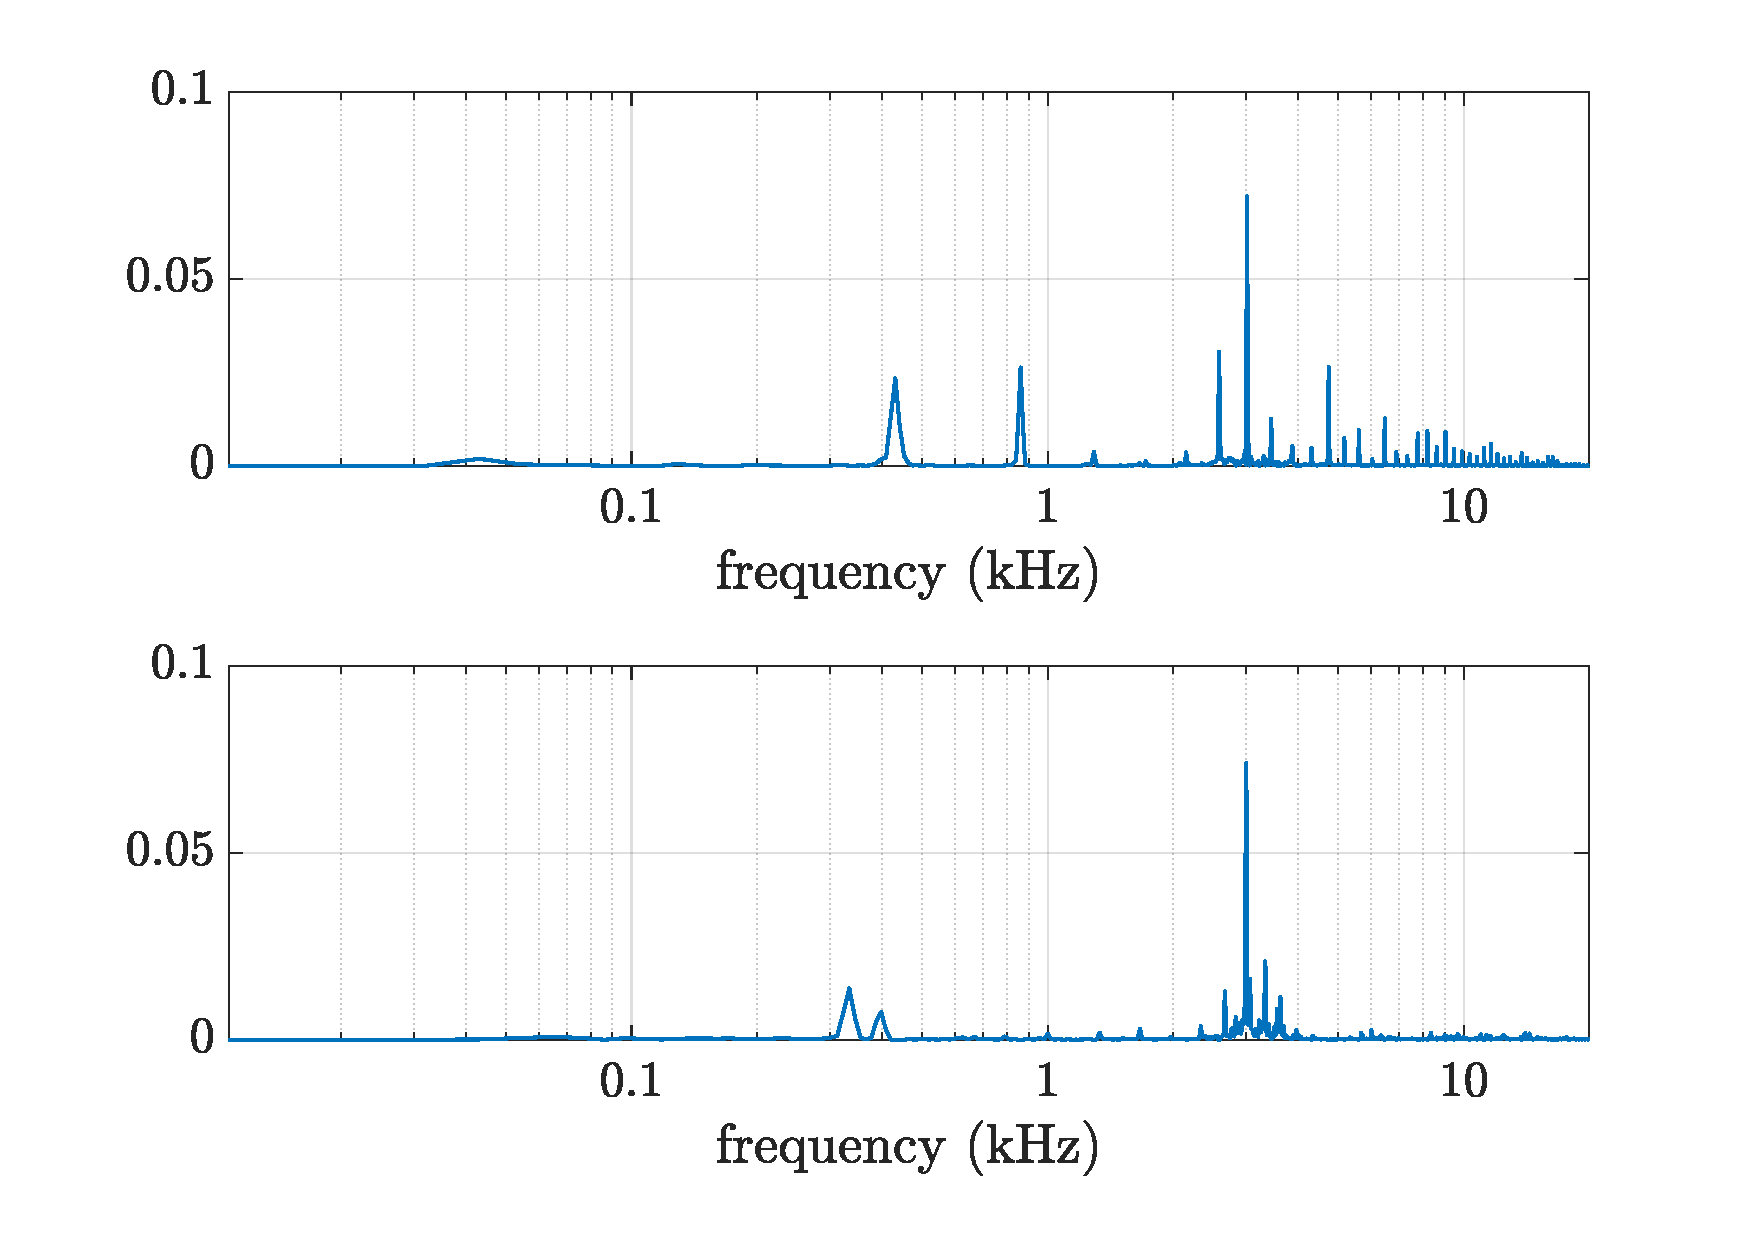
\includegraphics[width=\linewidth]{figures/Y_alert_TPR_-12_01.pdf}
        \caption{$TIR$ = -12}
        \label{fig:Y_alert-12}
    \end{subfigure}%
    \hfill
    \begin{subfigure}[t]{0.45\textwidth}
        \centering
        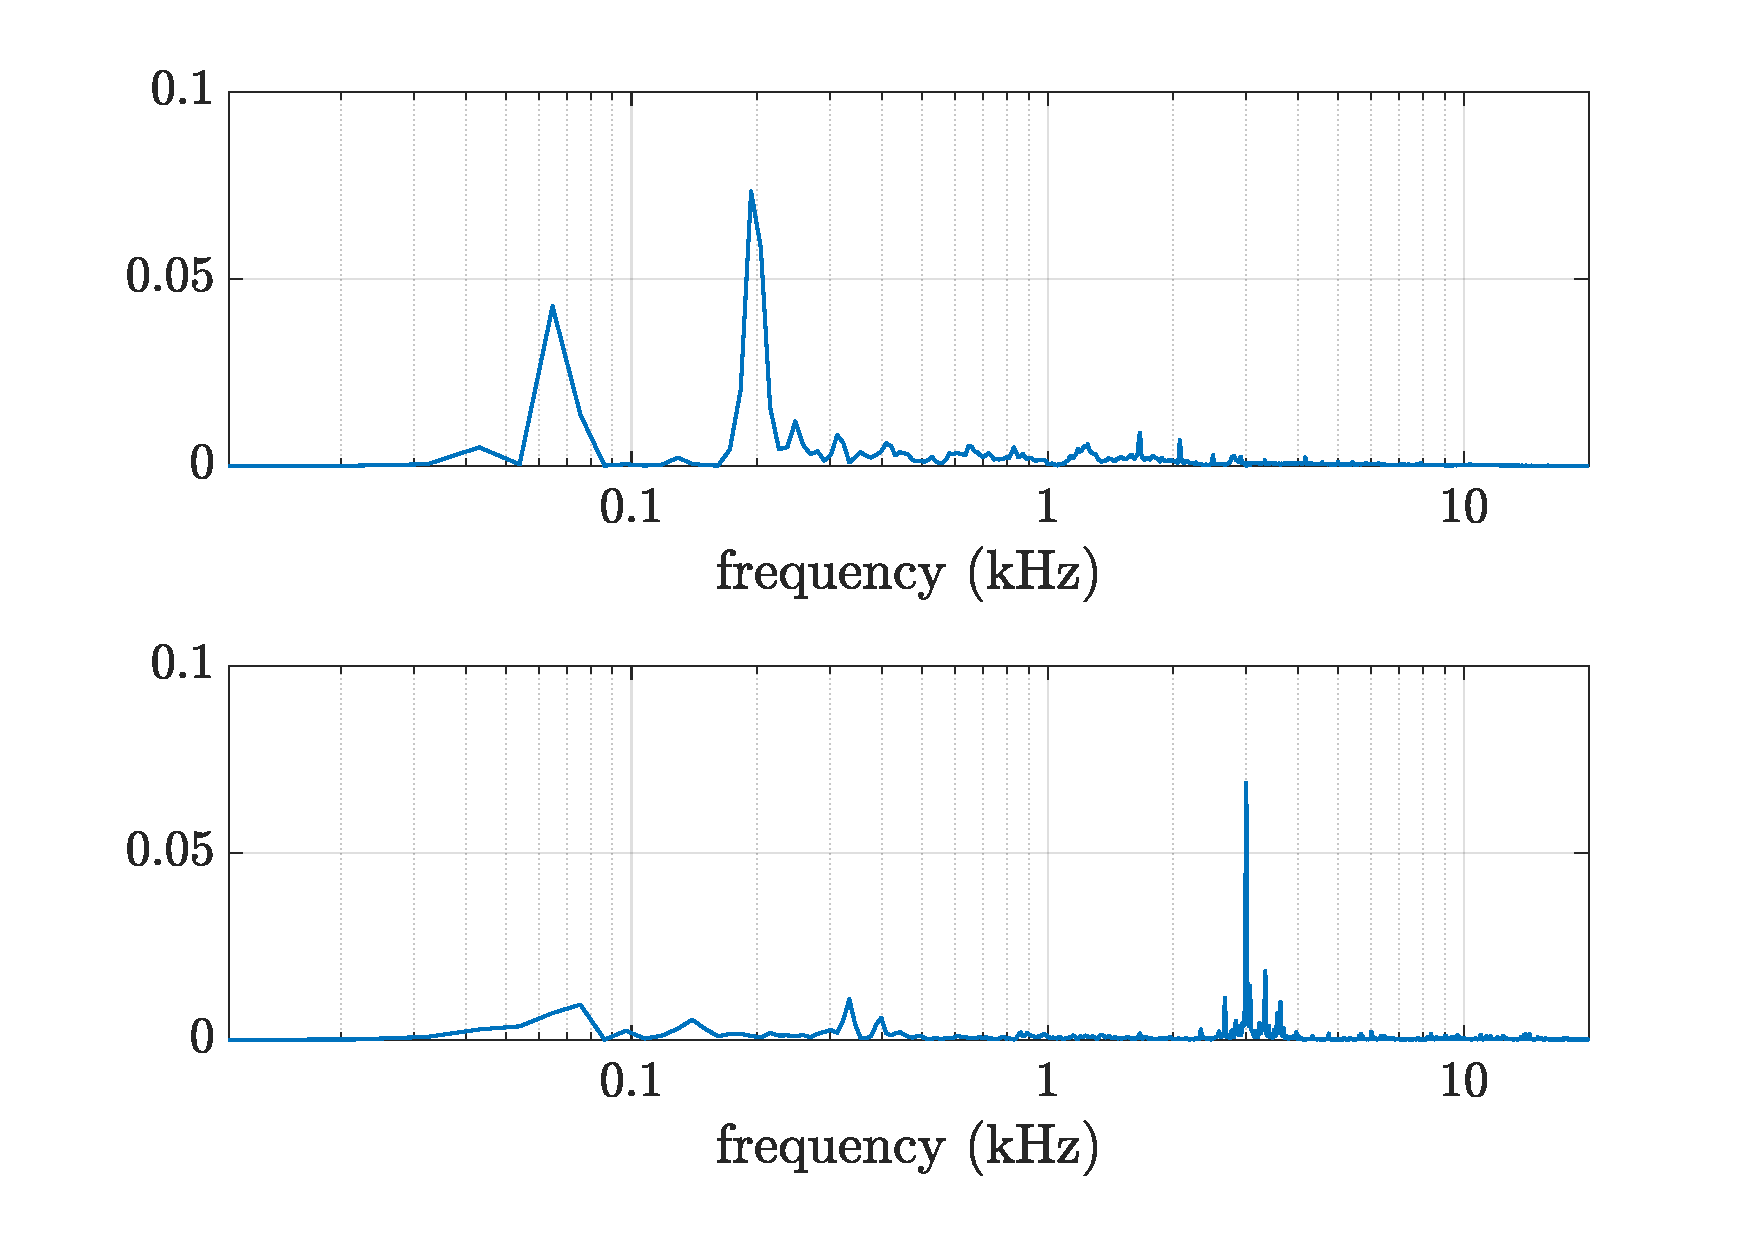
\includegraphics[width=\linewidth]{figures/Y_alert_TPR_12_01.pdf}
        \caption{$TIR$ = 12}
		\label{fig:Y_alert_12}
    \end{subfigure}
    \caption{$\mathbf{W_r}$ for an \textit{alert} scene}
\end{figure*}


The TI-NMF with a threshold fixed at $t = 0.54$, with a third octave spectral representation and $\beta$ = 2,  offers the lowest average results (Table \ref{tab:results}). According to each $TIR$, with the exception of $TIR$ = 0, all the mean errors are inferior to the baseline and supervised NMF errors. On the other hand, on low $TIR$, it does not succeed to be better than semi-supervised NMF.

Unlike supervised NMF, where $\mathbf{W}$ is fixed, and semi-supervised NMF, which combine a fixed dictionary with a mobile dictionary, TI-NMF's $\mathbf{W}$ is here update entirely to be adjusted to the scene and to adapt to the different sound environment. The closest elements of the \textit{traffic} component defined un $\mathbf{W_0}$ are then extracted to deduce the traffic signal. In Figure \ref{fig:dist_-12_12}, the similarity $D_{\theta}(\mathbf{W_0}||\mathbf{W})$ is displayed for 3 sub-classes for $TIR$ = [-12, 12].

\begin{figure}[t]
    \centering
    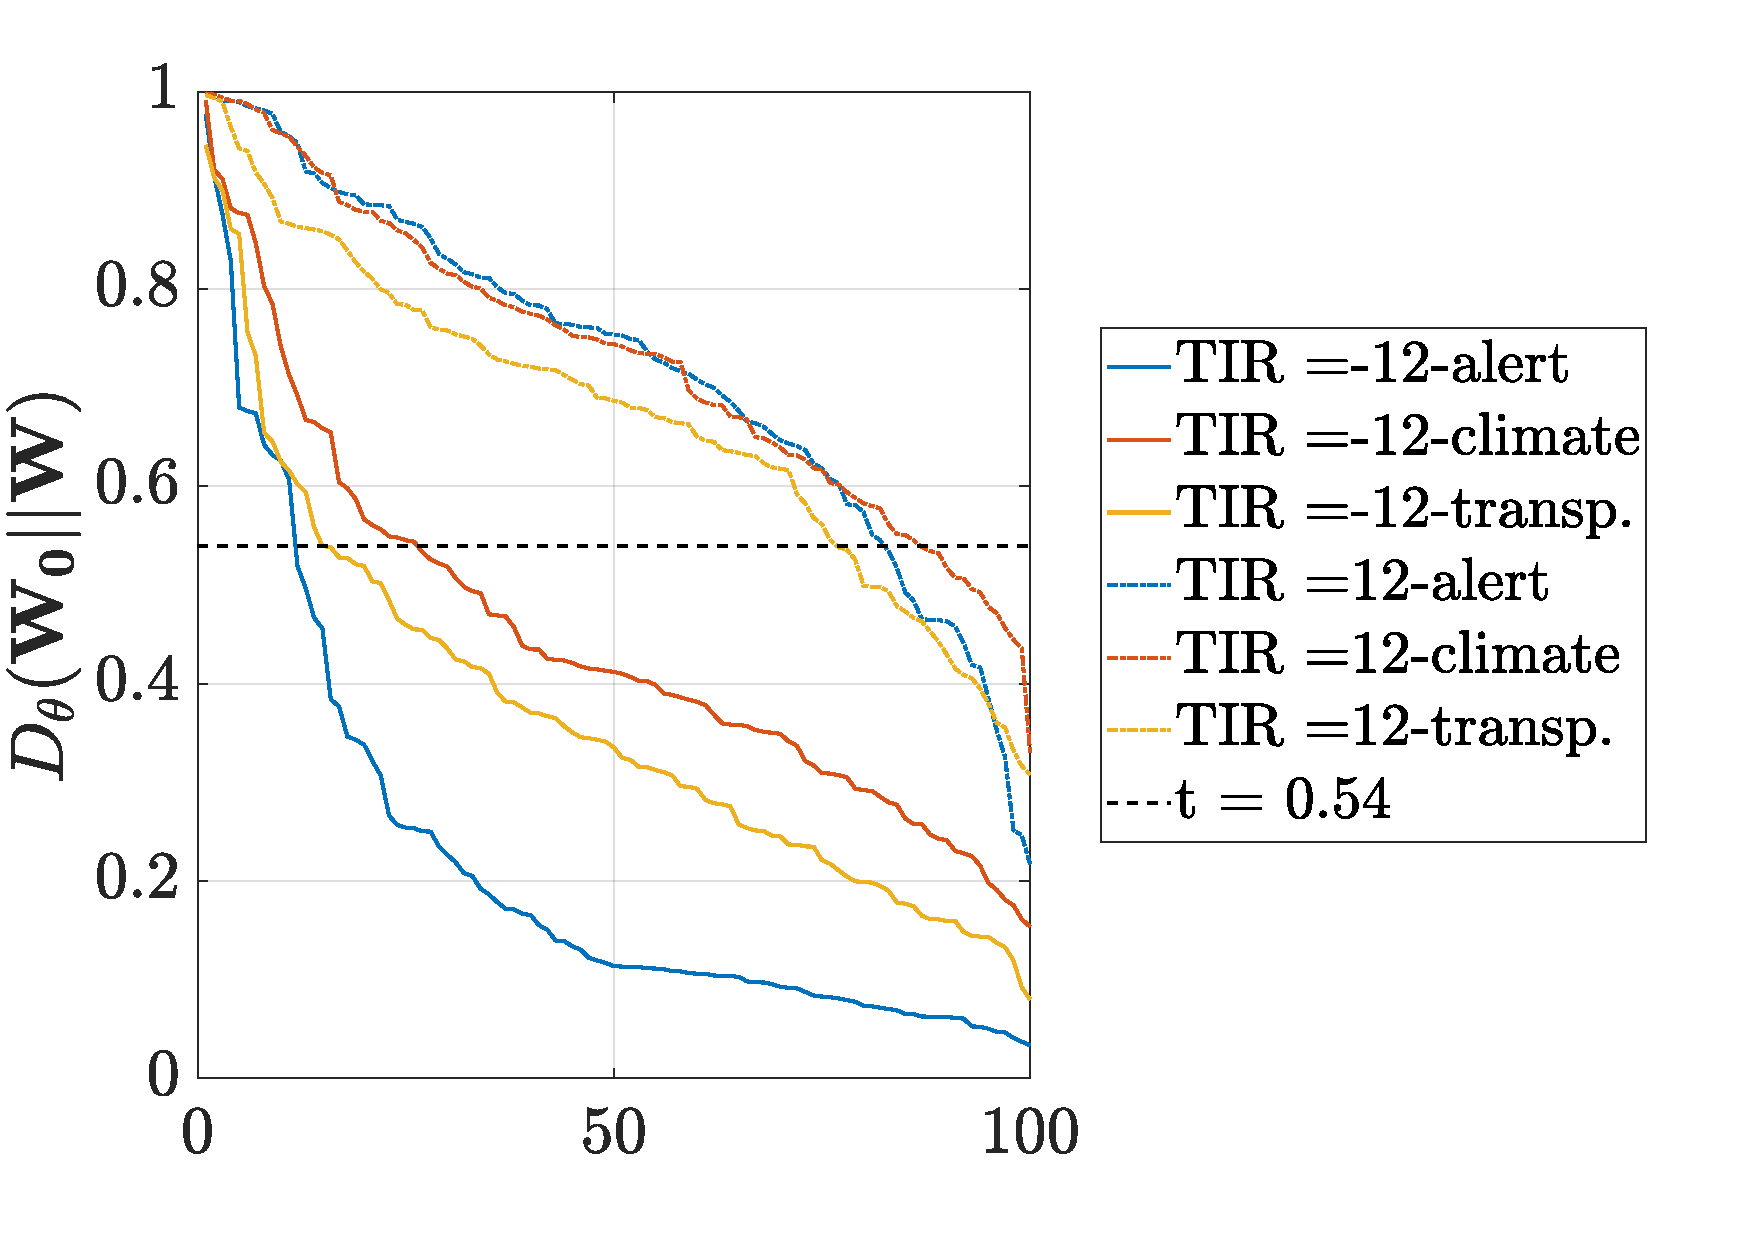
\includegraphics[width=\linewidth]{figures/dist_-12_12.pdf}
    \caption{Example of the similarity $\cos \theta$ for an sound mixture of the \textit{alert} sub-class for two $TIR$ and with the threshold $t$: $TIR = -12$ (a) and $TIR = 12$ (b)}
    \label{fig:dist_-12_12}
\end{figure}

For low $TIR$, with the thresholding, only a reduce number of $\mathbf{W}$ are considered as traffic components. In comparison to supervised results, this approach reduce significantly the error for the \textit{human} and \textit{transport} sub-classes.  However, for \textit{climate} and \textit{mechanics}, the error stay important (approfondir avec comparaison des niveau sonores trafic). On high $TIR$, as the traffic is the main sound source, the similarity of the initial dictionary and $\mathbf{W}$ is higher and allows to keep more elements. The kept elements are then more suited to the scenes than a fixed dictionary. So, the error, compare to supervised NMF, are better. In these cases, TI-NMF is the most powerful of the proposed methods.

\section{Conclusion}
ouvrir sur l'optimisation du seuil par plusieurs indicateurs (niveau sonore global ou en fréquence ? )\\
TI-NMF adapté pour d'autres sources sonores \\
Scènes grafic ensuite

\ml{non, une conclusion conclue, c'est tout.
rappel des resultats experimentaux et conclusion sur l'approche. Rappel des contributions et impact sur la communaute.
Petite ouverture sur le potentiel de l'approche: agnostique en terme de source, peut etre contraint temporellement citation, reste raisonable en terme de cout de calcul. }

\footnotesize
\bibliographystyle{unsrt}
\bibliography{bibliographie_applied}

\end{document}
